\documentclass[11pt]{article}
\usepackage{amssymb}
\usepackage{amsmath}
\usepackage{listings}
\usepackage[margin=1in,footskip=0.25in]{geometry}
\usepackage{xcolor}
\usepackage{graphicx}
\usepackage{subfig}
\usepackage{float}

\definecolor{mygrey}{gray}{.96} % Light Grey
\definecolor{BrickRed}{RGB}{120,0,0}
\lstset{
	language=C++,              % choose the language of the code ("language=Verilog" is popular as well)
   tabsize=3,							  % sets the size of the tabs in spaces (1 Tab is replaced with 3 spaces)
	basicstyle=\footnotesize,               % the size of the fonts that are used for the code
	numbers=left,                   % where to put the line-numbers
	numberstyle=\footnotesize,              % the size of the fonts that are used for the line-numbers
	stepnumber=1,                   % the step between two line-numbers. If it's 1 each line will be numbered
	numbersep=5pt,                  % how far the line-numbers are from the code
	backgroundcolor=\color{mygrey}, % choose the background color. You must add \usepackage
	showspaces=false,              % show spaces adding particular underscores
	showstringspaces=false,        % underline spaces within strings
	showtabs=false,                % show tabs within strings adding particular underscores
	frame=single,	                 % adds a frame around the code
	tabsize=3,	                    % sets default tabsize to 2 spaces
	captionpos=b,                   % sets the caption-position to bottom
	breaklines=true,                % sets automatic line breaking
	breakatwhitespace=false,        % sets if automatic breaks should only happen at whitespace
	%escapeinside={\%*}{*)},        % if you want to add a comment within your code
	commentstyle=\color{BrickRed}   % sets the comment style
}
%Gummi|065|=)
\title{\Huge{\textbf{\underline{Monte Carlo Simulation: Assignment 2}}}}
\author{Yash Vanjani\\
		Roll No:140123046\\
		}
\date{26/01/2016}
\begin{document}
\maketitle
\Large{\textbf{\underline{Question 1}}}\\\\
Implement the linear congruence generator $x_{i+1}=ax_i mod m$ to generate a sequence $x_i$ and hence uniform random numbers $u_i$. Make use of the following values of a and mP: (a)$a=16807$ and $m=2^{31}-1$. (b)$a=406932$ and $m=214783399$. (c) $a=40014$ and $m=2147483563$.\\
Group the values into equidistant ranges for the values of $u_i$. Tabulate the proportions
and draw a bar diagram for the above. What do you observe ? Do it for 1000, 10000
and 100000 values.\\
For part (a) do the following: Plot the values$(u_i,u_{i+1})$ on a unit square. Now, zoom into the range $u_i\in[0,0.001]$. What are your observations?\\\\
\Large{\textbf{\underline{Solution}}}\\\\
\underline{C++ Code:}
\begin{lstlisting} [frame=single]
#include <iostream>
#include <fstream>
#include <cmath>

using namespace std;

int main()
{
	ofstream myfile;
	myfile.open("output.txt", ios::app);
	long int x[100000];
	long int a[3];
	long int m[3];
	long int q,r,k,b;
	float u[3][3][100000];
	int f[3][3][20];
	a[0]=16807;
	a[1]=40692;
	a[2]=40014;
	m[0]=(pow(2,31)-1);
	m[1]=2147483399;
	m[2]=2147483563;
	int i,j,l;
	long int n[3]={1000,10000,100000};

	for(i=0;i<3;i++) //loop for n[i]
	{
		for(j=0;j<3;j++) //loop for a[i],m[i]
		{
			x[0]=12345;
			for(l=0;l<n[i]-1;l++) //loop for calculating x[i]
			{
				q=m[j]/a[j];
				r=m[j] % a[j];
				k=x[l]/q;
				b=x[l]-(k*q);
				x[l+1]=(a[j]*b)-(k*r);
				if (x[l+1]<0)
					x[l+1]=x[l+1]+m[j];
				u[i][j][l+1]=float(x[l+1])/float(m[j]);
			}
			u[i][j][0]=float(x[0])/float(m[j]);
			for(l=0;l<n[i];l++)
            {
                if(u[i][j][l]>=0 && u[i][j][l]<0.05)
                    f[i][j][0]++;
                if(u[i][j][l]>=0.05 && u[i][j][l]<0.10)
                    f[i][j][1]++;
                if(u[i][j][l]>=0.10 && u[i][j][l]<0.15)
                    f[i][j][2]++;
                if(u[i][j][l]>=0.15 && u[i][j][l]<0.20)
                    f[i][j][3]++;
                if(u[i][j][l]>=0.20 && u[i][j][l]<0.25)
                    f[i][j][4]++;
                if(u[i][j][l]>=0.25 && u[i][j][l]<0.30)
                    f[i][j][5]++;
                if(u[i][j][l]>=0.30 && u[i][j][l]<0.35)
                    f[i][j][6]++;
                if(u[i][j][l]>=0.35 && u[i][j][l]<0.40)
                    f[i][j][7]++;
                if(u[i][j][l]>=0.40 && u[i][j][l]<0.45)
                    f[i][j][8]++;
                if(u[i][j][l]>=0.45 && u[i][j][l]<0.50)
                    f[i][j][9]++;
                if(u[i][j][l]>=0.50 && u[i][j][l]<0.55)
                    f[i][j][10]++;
                if(u[i][j][l]>=0.55 && u[i][j][l]<0.60)
                    f[i][j][11]++;
                if(u[i][j][l]>=0.60 && u[i][j][l]<0.65)
                    f[i][j][12]++;
                if(u[i][j][l]>=0.65 && u[i][j][l]<0.70)
                    f[i][j][13]++;
                if(u[i][j][l]>=0.70 && u[i][j][l]<0.75)
                    f[i][j][14]++;
                if(u[i][j][l]>=0.75 && u[i][j][l]<0.80)
                    f[i][j][15]++;
                if(u[i][j][l]>=0.80 && u[i][j][l]<0.85)
                    f[i][j][16]++;
                if(u[i][j][l]>=0.85 && u[i][j][l]<0.90)
                    f[i][j][17]++;
                if(u[i][j][l]>=0.90 && u[i][j][l]<0.95)
                    f[i][j][18]++;
                if(u[i][j][l]>=0.95 && u[i][j][l]<=1)
                    f[i][j][19]++;
 
            }
		}

	}



	for(i=0;i<3;i++) //loop for n[i]
	{
		myfile<<"For n="<<n[i]<<"\n";
		for(j=0;j<3;j++) //loop for a[i],m[i]
		{
			myfile<<"		For a="<<a[j]<<" and m="<<m[j]<<"\n";
			for(l=0;l<20;l++) //loop for calculating x[i]
			{
				
				myfile<<f[i][j][l]<<"\n";
			}
		}
		cout<<"\n";

	}
	myfile.close();

	myfile.open("2dplot1.txt", ios::app);
	for(l=0;l<999;l++)
	{
		myfile<<u[0][0][l]<<"		"<<u[0][0][l+1]<<"\n";
	}
	myfile.close();

	myfile.open("2dplot2.txt", ios::app);
	for(l=0;l<9999;l++)
	{
		myfile<<u[1][0][l]<<"		"<<u[1][0][l+1]<<"\n";
	}
	myfile.close();

	myfile.open("2dplot3.txt", ios::app);
	for(l=0;l<99999;l++)
	{
		myfile<<u[2][0][l]<<"		"<<u[2][0][l+1]<<"\n";
	}
	myfile.close();

	myfile.open("2dplot_zoom1.txt", ios::app);
	for(l=0;l<999;l++)
	{
		if(u[0][0][l]<=0.001 )//&& u[0][0][l+1]<=0.001)
			myfile<<u[0][0][l]<<"		"<<u[0][0][l+1]<<"\n";
	}
	myfile.close();

	myfile.open("2dplot_zoom2.txt", ios::app);
	for(l=0;l<9999;l++)
	{
		if(u[1][0][l]<=0.001 )//&& u[1][0][l+1]<=0.001)
			myfile<<u[1][0][l]<<"		"<<u[1][0][l+1]<<"\n";
	}
	myfile.close();

	myfile.open("2dplot_zoom3.txt", ios::app);
	for(l=0;l<99999;l++)
	{
		if(u[2][0][l]<=0.001 )//&& u[2][0][l+1]<=0.001)
			myfile<<u[2][0][l]<<"		"<<u[2][0][l+1]<<"\n";
	}
	myfile.close();
}

\end{lstlisting}
\underline{Output:}
\begin{lstlisting}
For n=1000
		For a=16807 and m=2147483647
54
51
41
52
59
45
65
50
58
47
45
49
51
45
54
44
41
49
55
45
		For a=40692 and m=2147483399
48
51
54
47
57
68
56
52
52
36
46
32
56
44
53
49
42
49
54
54
		For a=40014 and m=2147483563
51
50
47
49
53
49
50
48
50
41
58
50
35
51
41
54
50
50
59
64
For n=10000
		For a=16807 and m=2147483647
498
502
480
490
474
511
513
535
487
485
470
517
530
501
474
503
478
527
518
507
		For a=40692 and m=2147483399
503
507
540
488
486
469
506
505
514
549
504
484
514
477
507
452
485
495
497
518
		For a=40014 and m=2147483563
470
489
484
530
516
517
526
479
491
518
501
486
471
522
482
499
499
491
521
508
For n=100000
		For a=16807 and m=2147483647
5002
4973
4987
5055
4932
5054
4952
5127
4983
5018
4972
4967
5028
4975
5046
4978
4887
5101
4856
5107
		For a=40692 and m=2147483399
4990
5112
5140
4962
4895
5070
5062
4943
4997
5119
4939
4979
4954
4984
4911
4976
5055
4967
4954
4991
		For a=40014 and m=2147483563
4933
4889
4840
5086
5037
5106
5064
4889
5039
4990
5126
4986
4989
5010
4893
4949
5114
4961
5003
5096 
\end{lstlisting}
\newpage
\underline{\\Histograms:}
\begin{figure}[H]
	\centering
	\subfloat{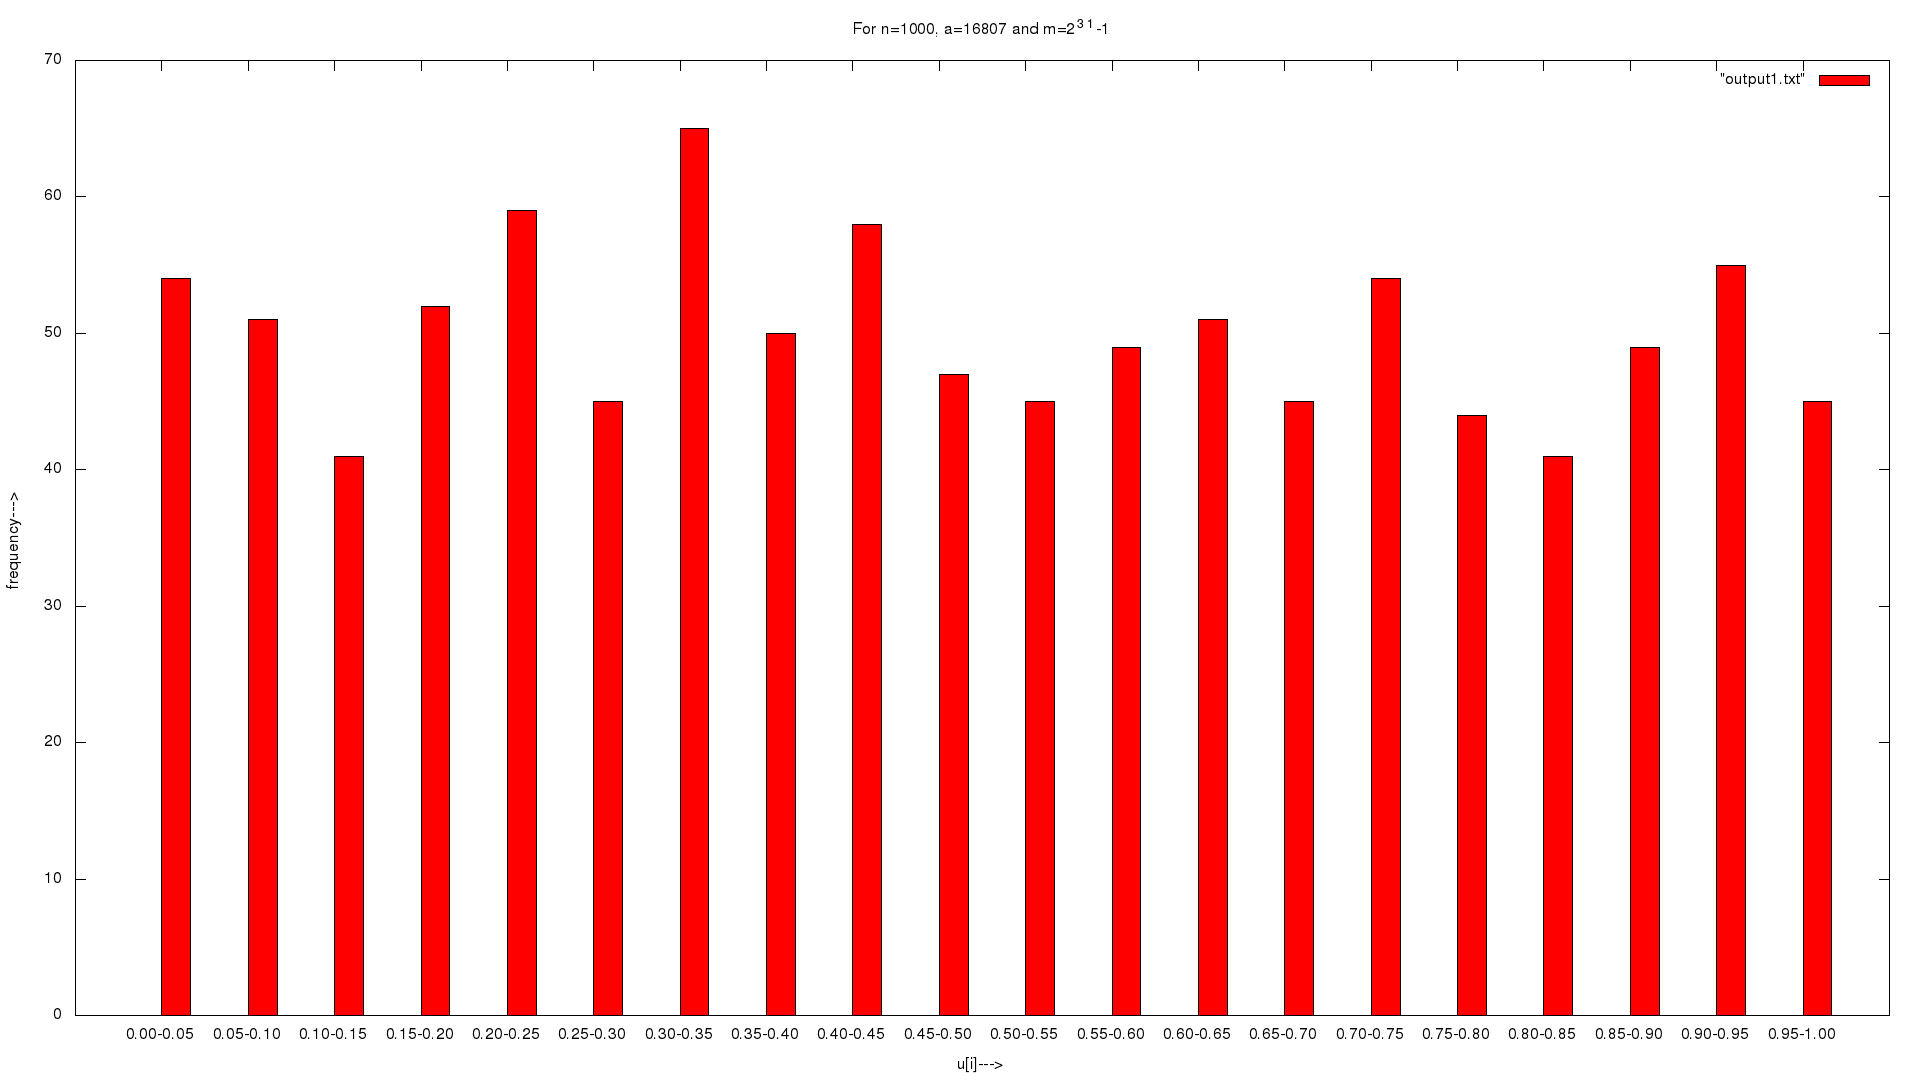
\includegraphics[width=1.0\textwidth]{q1_n1_freq1.png}}
	\caption{Frequency graph for a=16807, $m=2^{31}-1$ for 1000 random numbers}
\end{figure}
\begin{figure}[H]
	\centering
	\subfloat{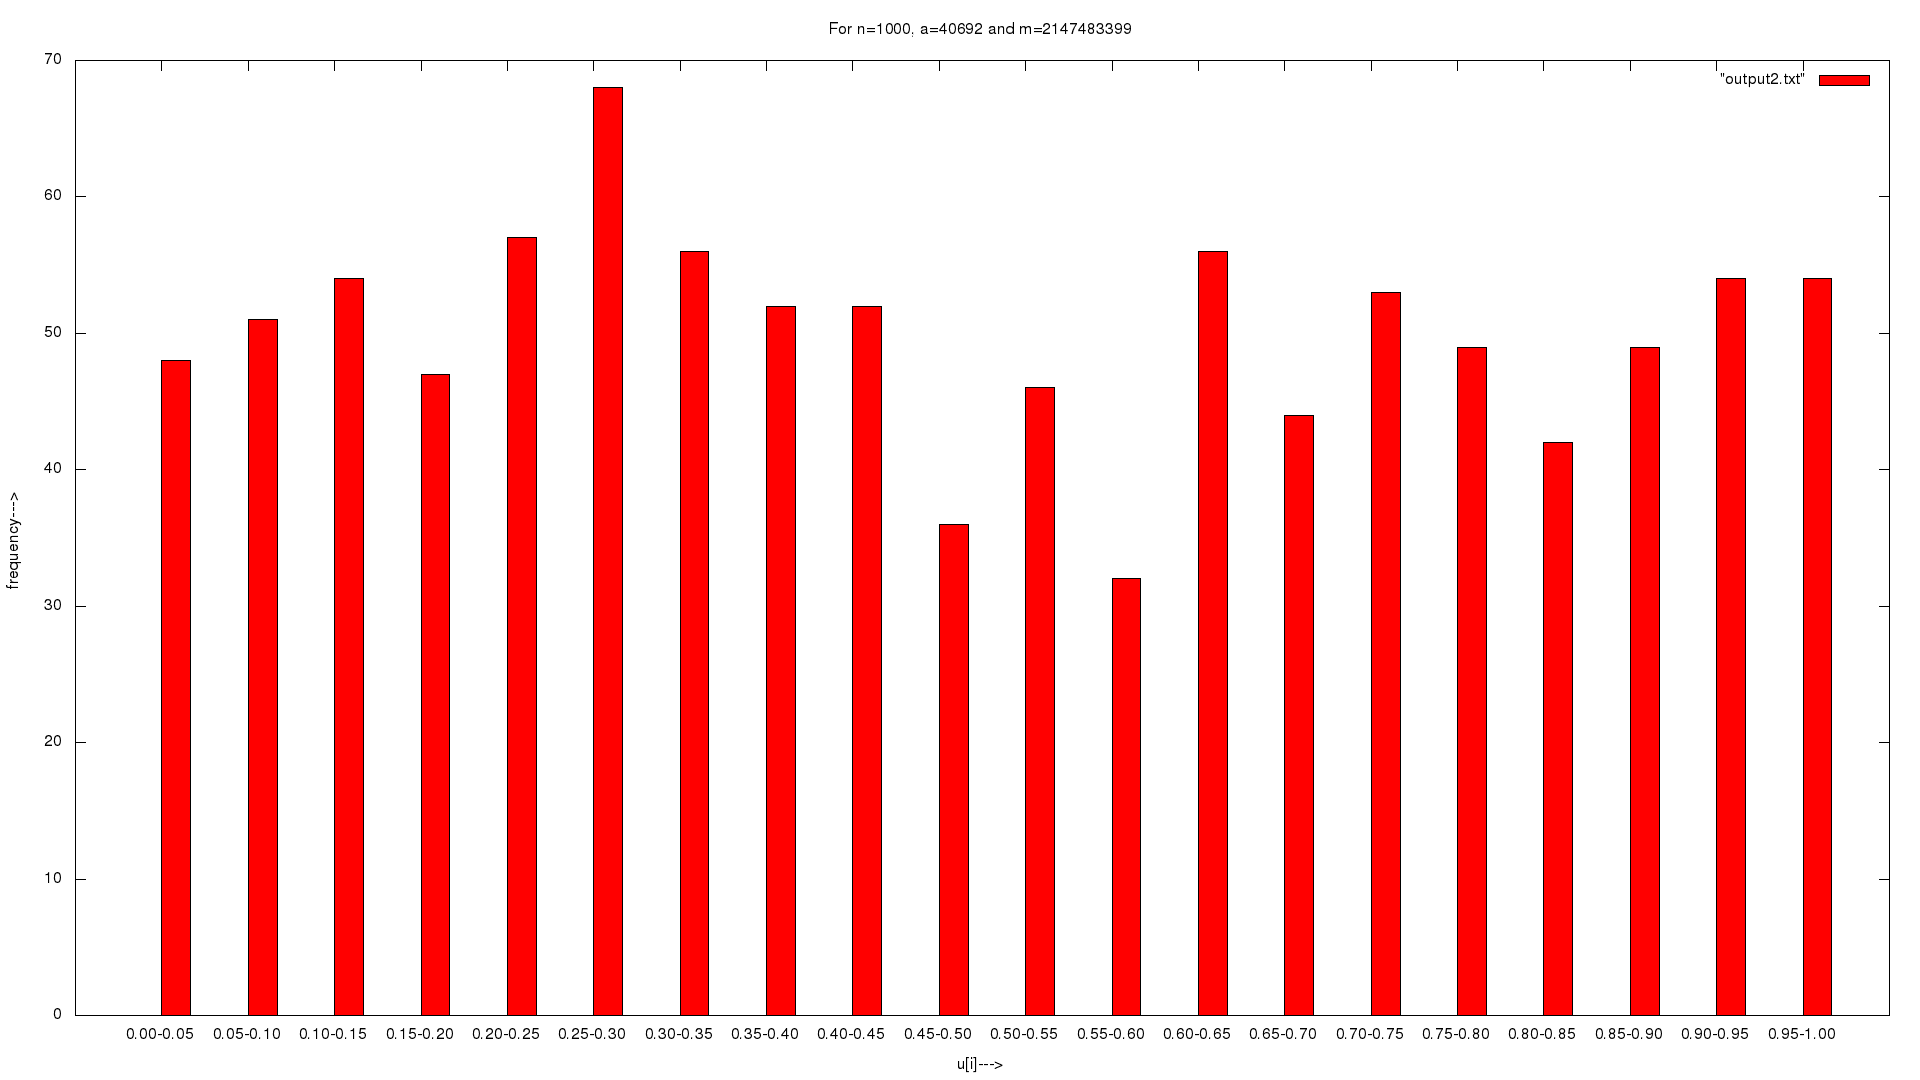
\includegraphics[width=1.0\textwidth]{q1_n1_freq2.png}}
	\caption{Frequency graph for a=40692, $m=2147483399$ for 1000 random numbers}
\end{figure}
\begin{figure}[H]
	\centering
	\subfloat{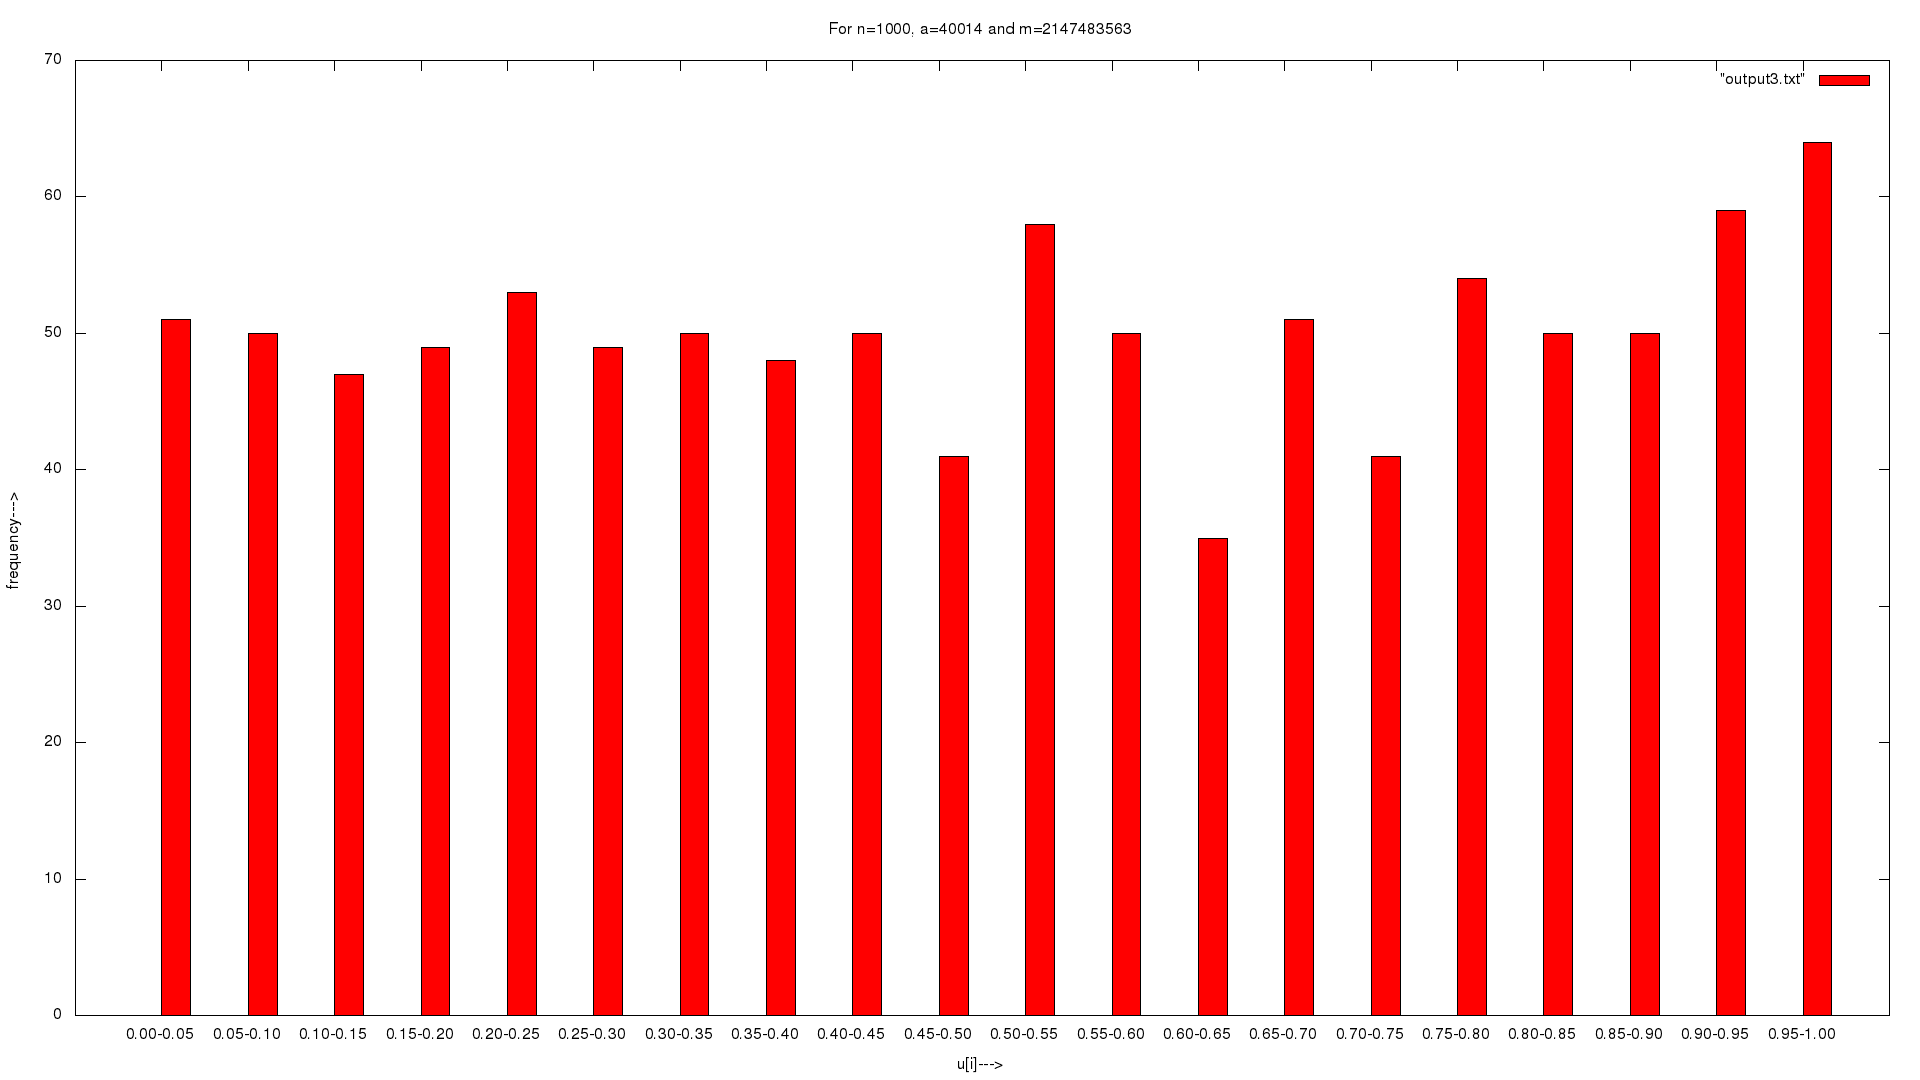
\includegraphics[width=1.0\textwidth]{q1_n1_freq3.png}}
	\caption{Frequency graph for a=40014, $m=2147483563$ for 1000 random numbers}
\end{figure}
\begin{figure}[H]
	\centering
	\subfloat{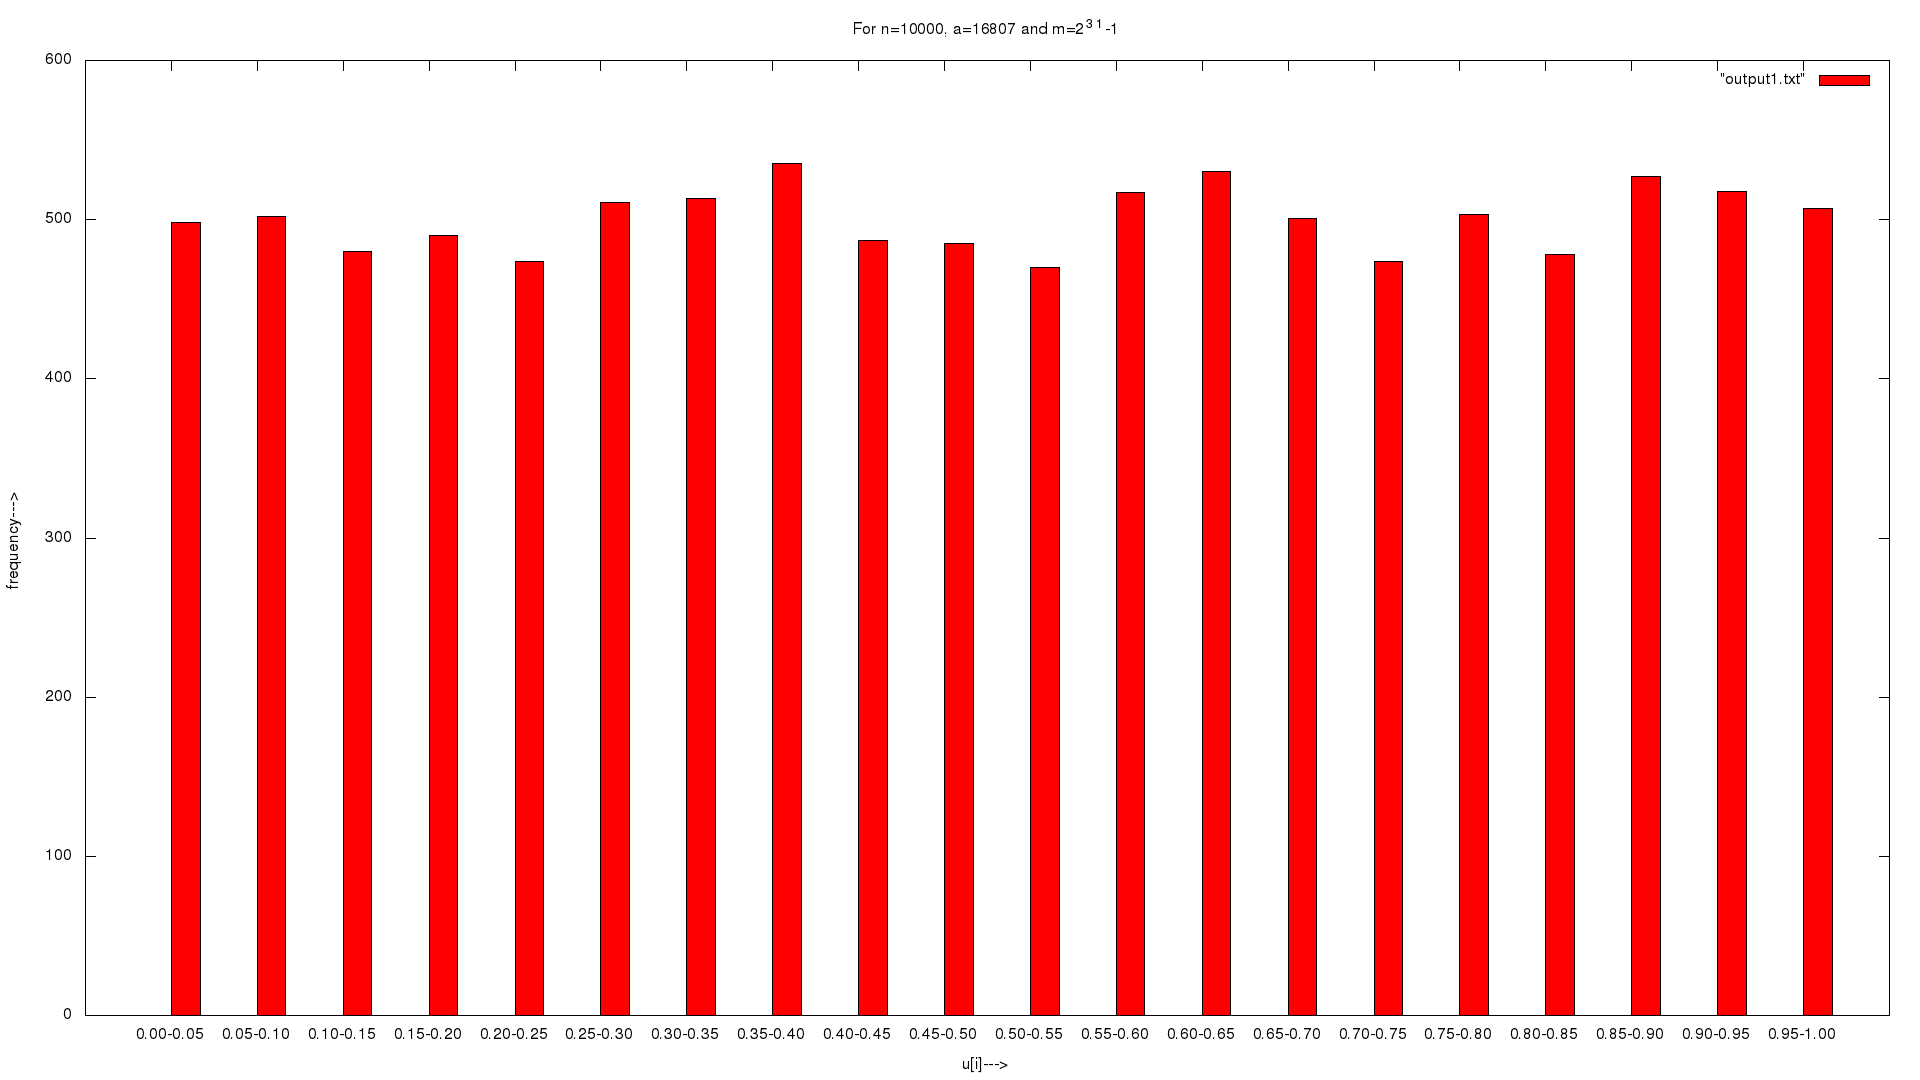
\includegraphics[width=1.0\textwidth]{q1_n2_freq1.png}}
	\caption{Frequency graph for a=16807, $m=2^{31}-1$ for 10000 random numbers}
\end{figure}
\begin{figure}[H]
	\centering
	\subfloat{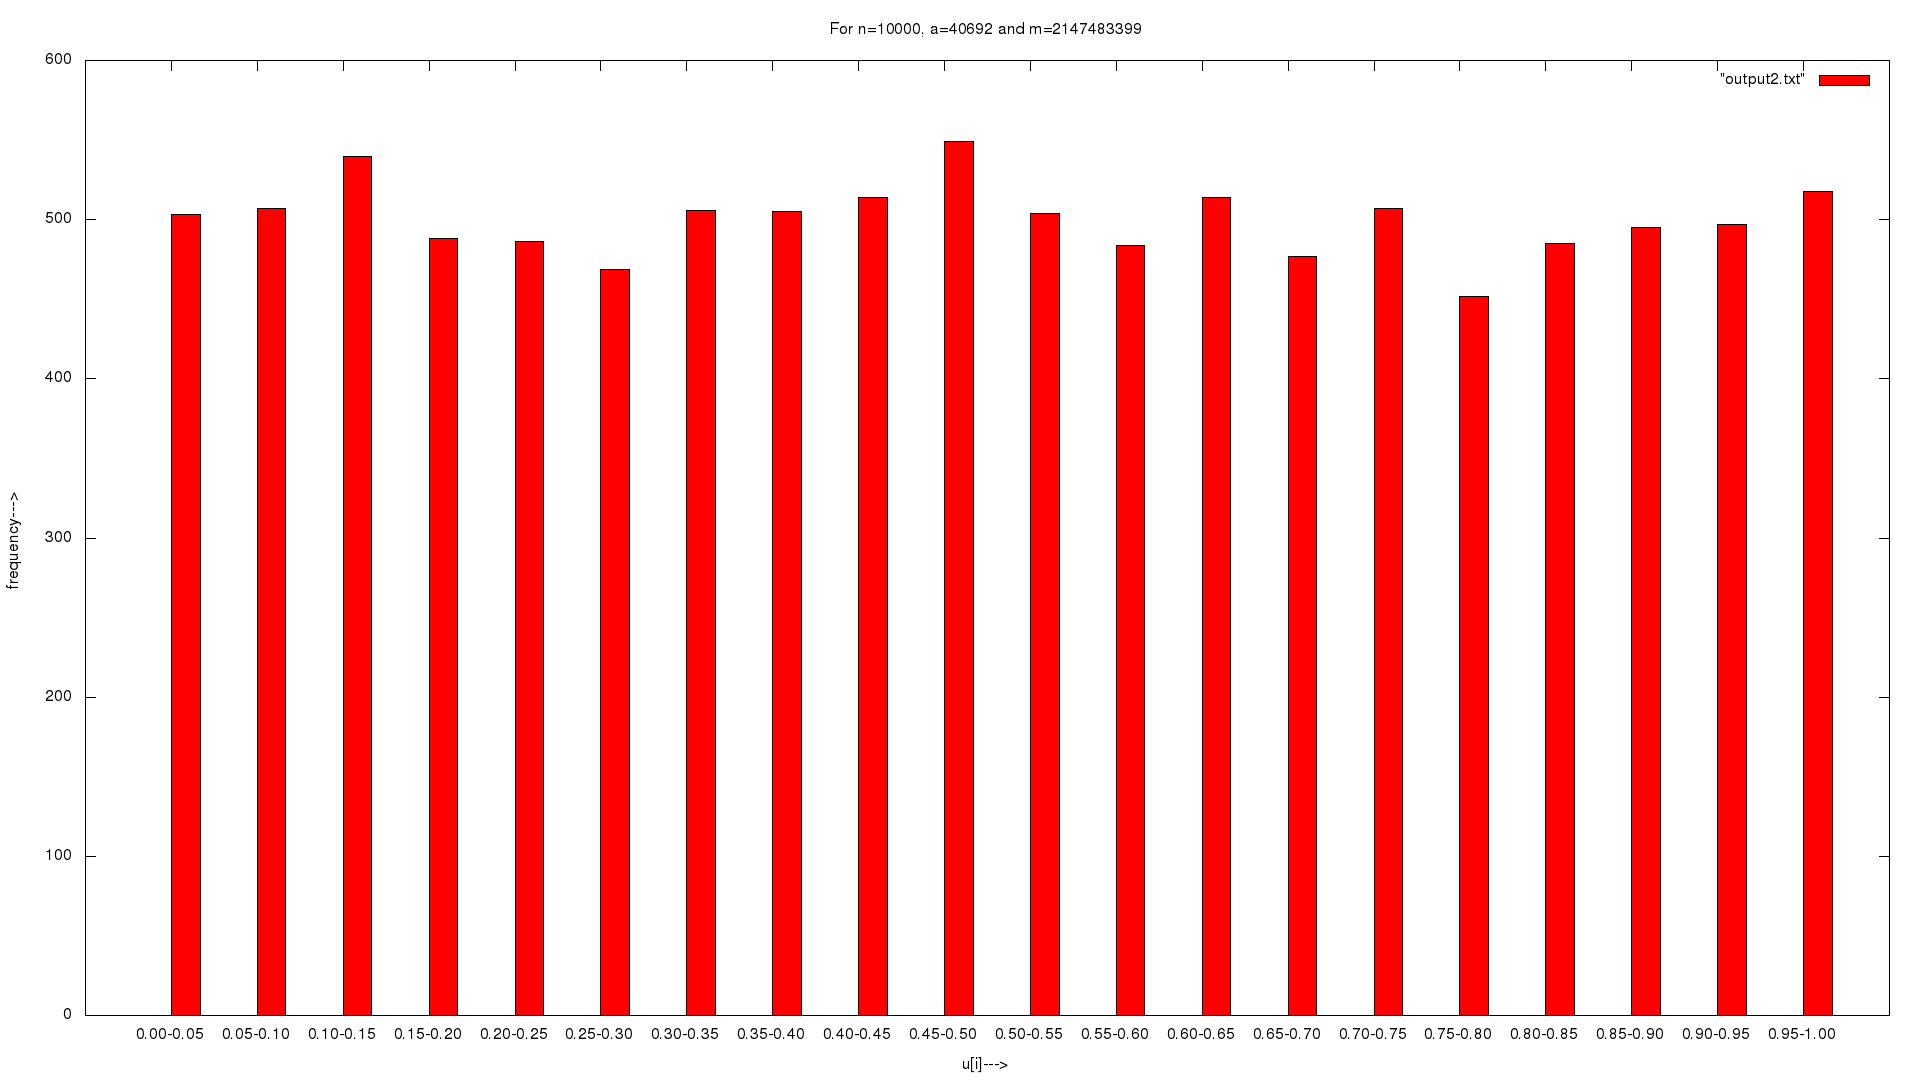
\includegraphics[width=1.0\textwidth]{q1_n2_freq2.png}}
	\caption{Frequency graph for a=40692, $m=2147483399$ for 10000 random numbers}
\end{figure}
\begin{figure}[H]
	\centering
	\subfloat{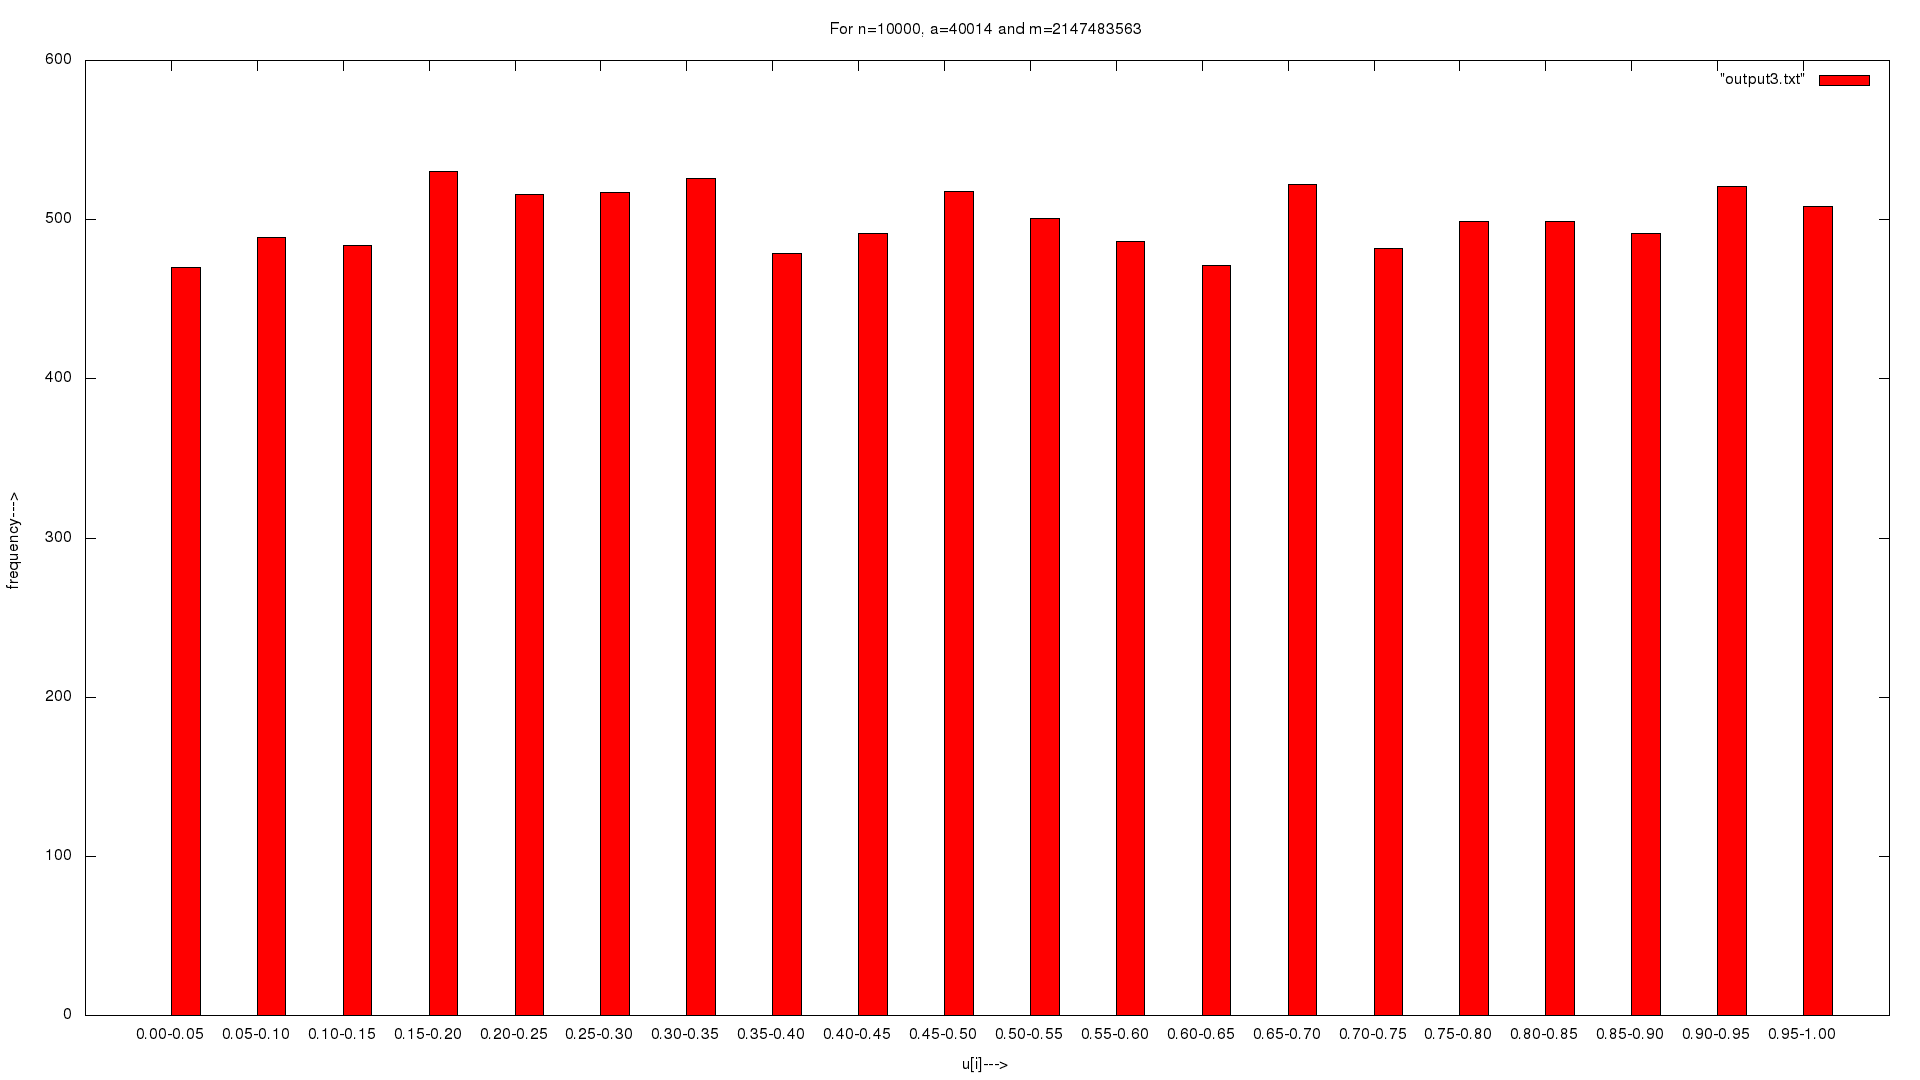
\includegraphics[width=1.0\textwidth]{q1_n2_freq3.png}}
	\caption{Frequency graph for a=40014, $m=2147483563$ for 10000 random numbers}
\end{figure}
\begin{figure}[H]
	\centering
	\subfloat{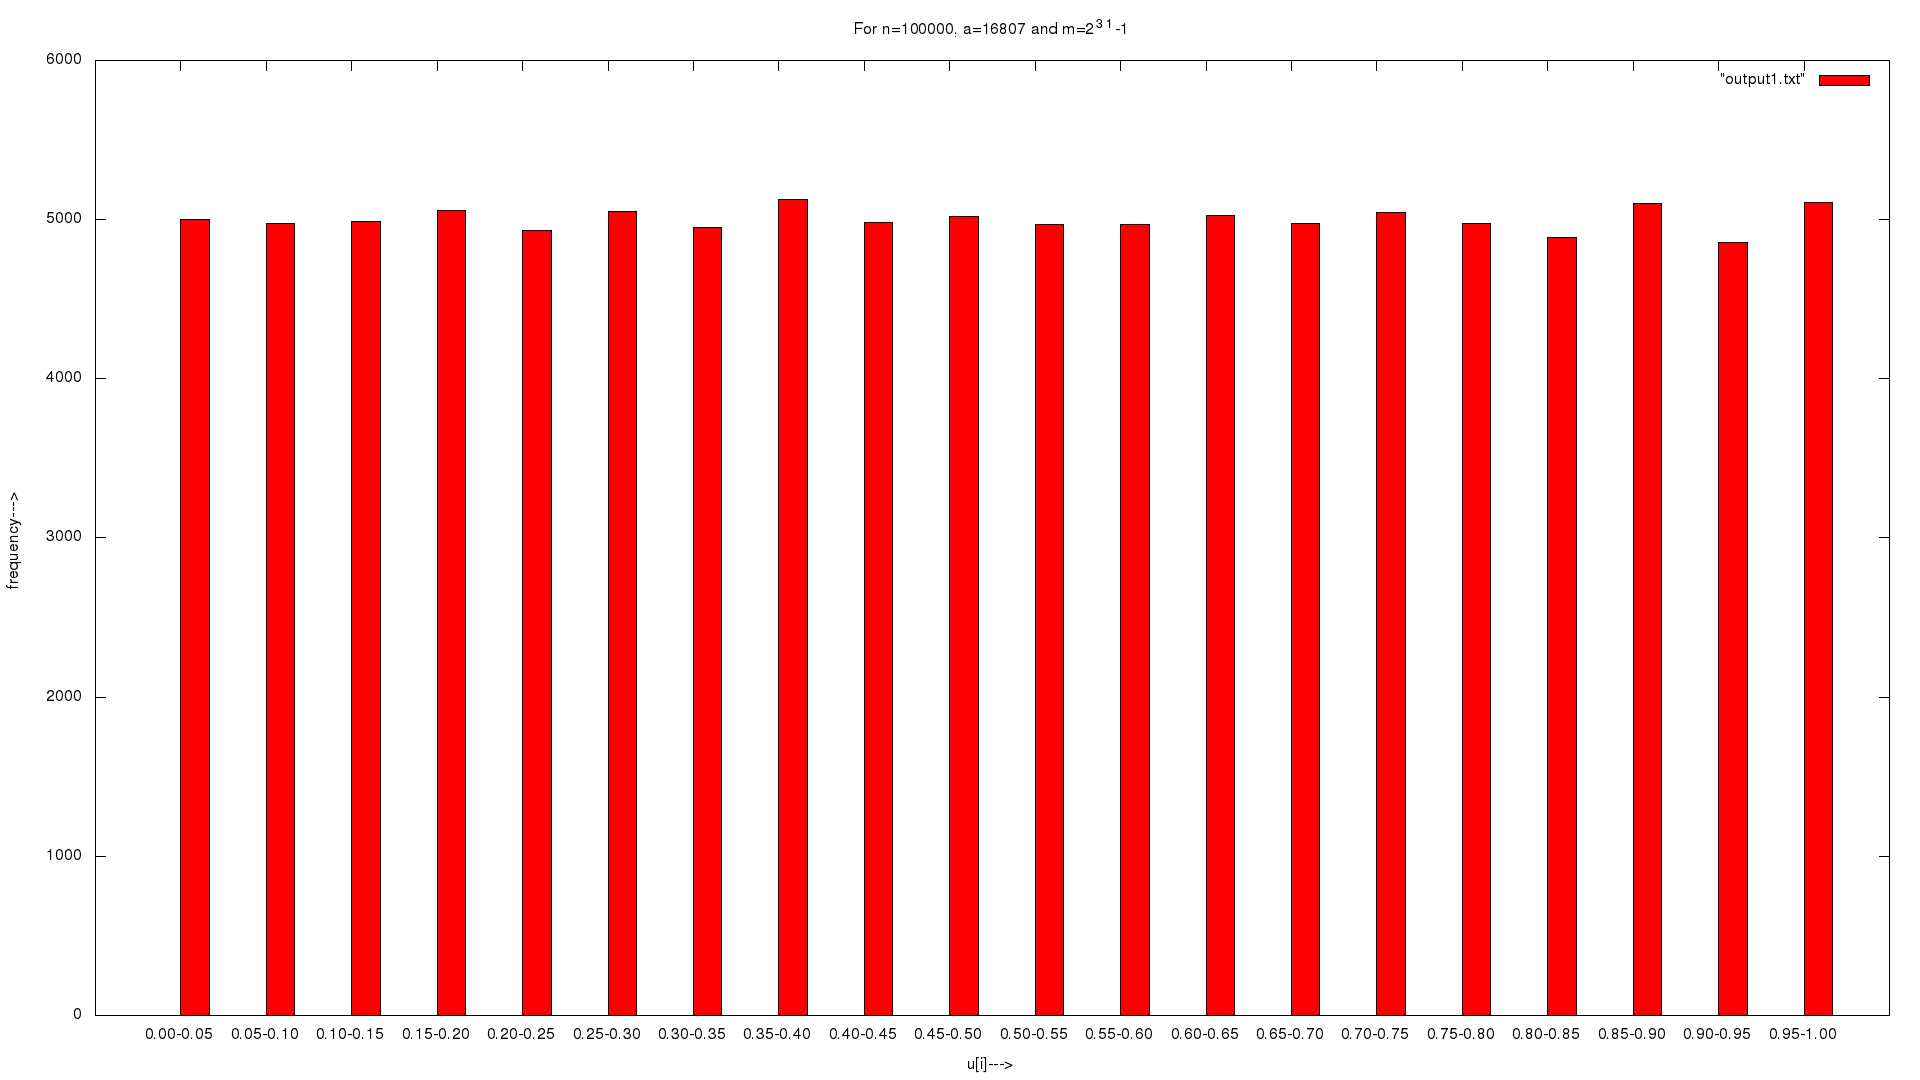
\includegraphics[width=1.0\textwidth]{q1_n3_freq1.png}}
	\caption{Frequency graph for a=16807, $m=2^{31}-1$ for 100000 random numbers}
\end{figure}
\begin{figure}[H]
	\centering
	\subfloat{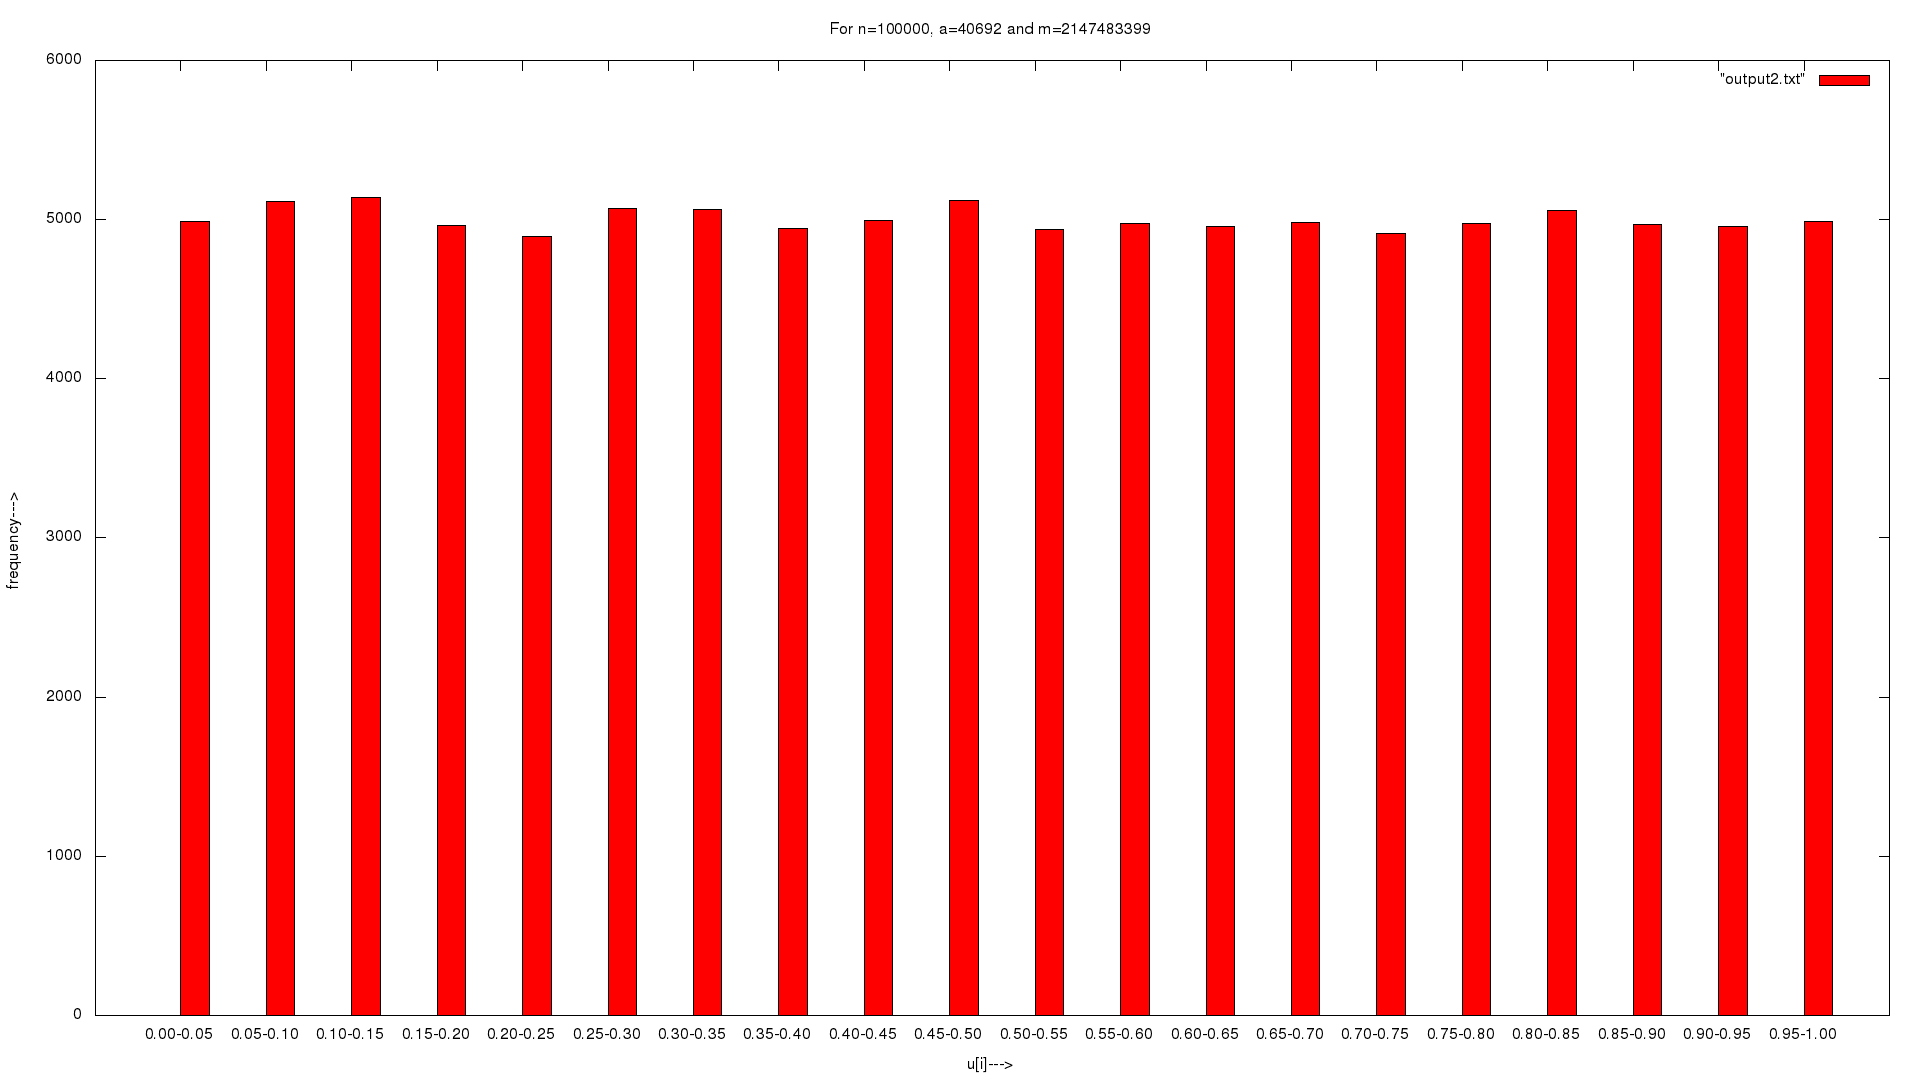
\includegraphics[width=1.0\textwidth]{q1_n3_freq2.png}}
	\caption{Frequency graph for a=40692, $m=2147483399$ for 100000 random numbers}
\end{figure}
\begin{figure}[H]
	\centering
	\subfloat{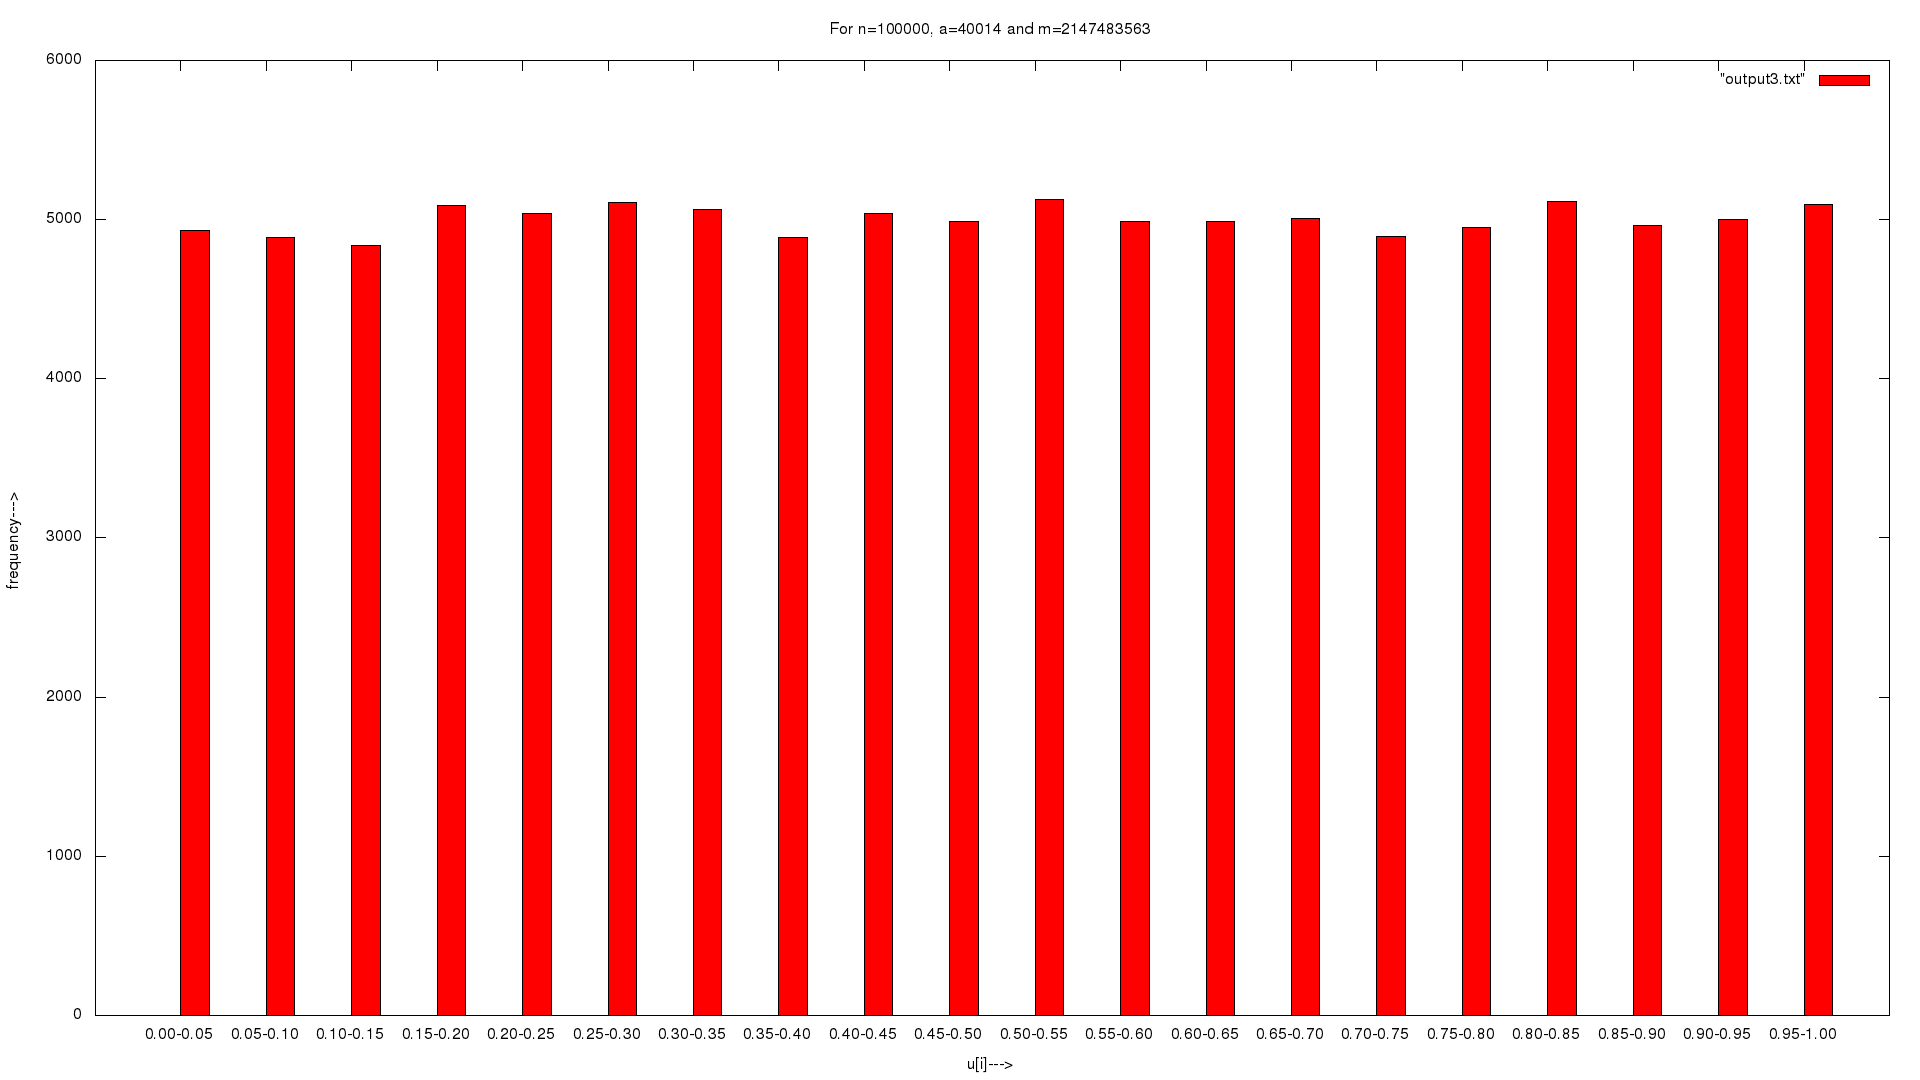
\includegraphics[width=1.0\textwidth]{q1_n3_freq3.png}}
	\caption{Frequency graph for a=40014, $m=2147483563$ for 100000 random numbers}
\end{figure}
\underline{Observations:}
\begin{itemize}
\item The height of bars in the bar graph tend to equal as the number of random numbers generated are increased thus showing that the random numbers generated become more uniform.
\end{itemize}
\newpage
\underline{2D-Plots:}
\begin{figure}[H]
	\centering
	\subfloat{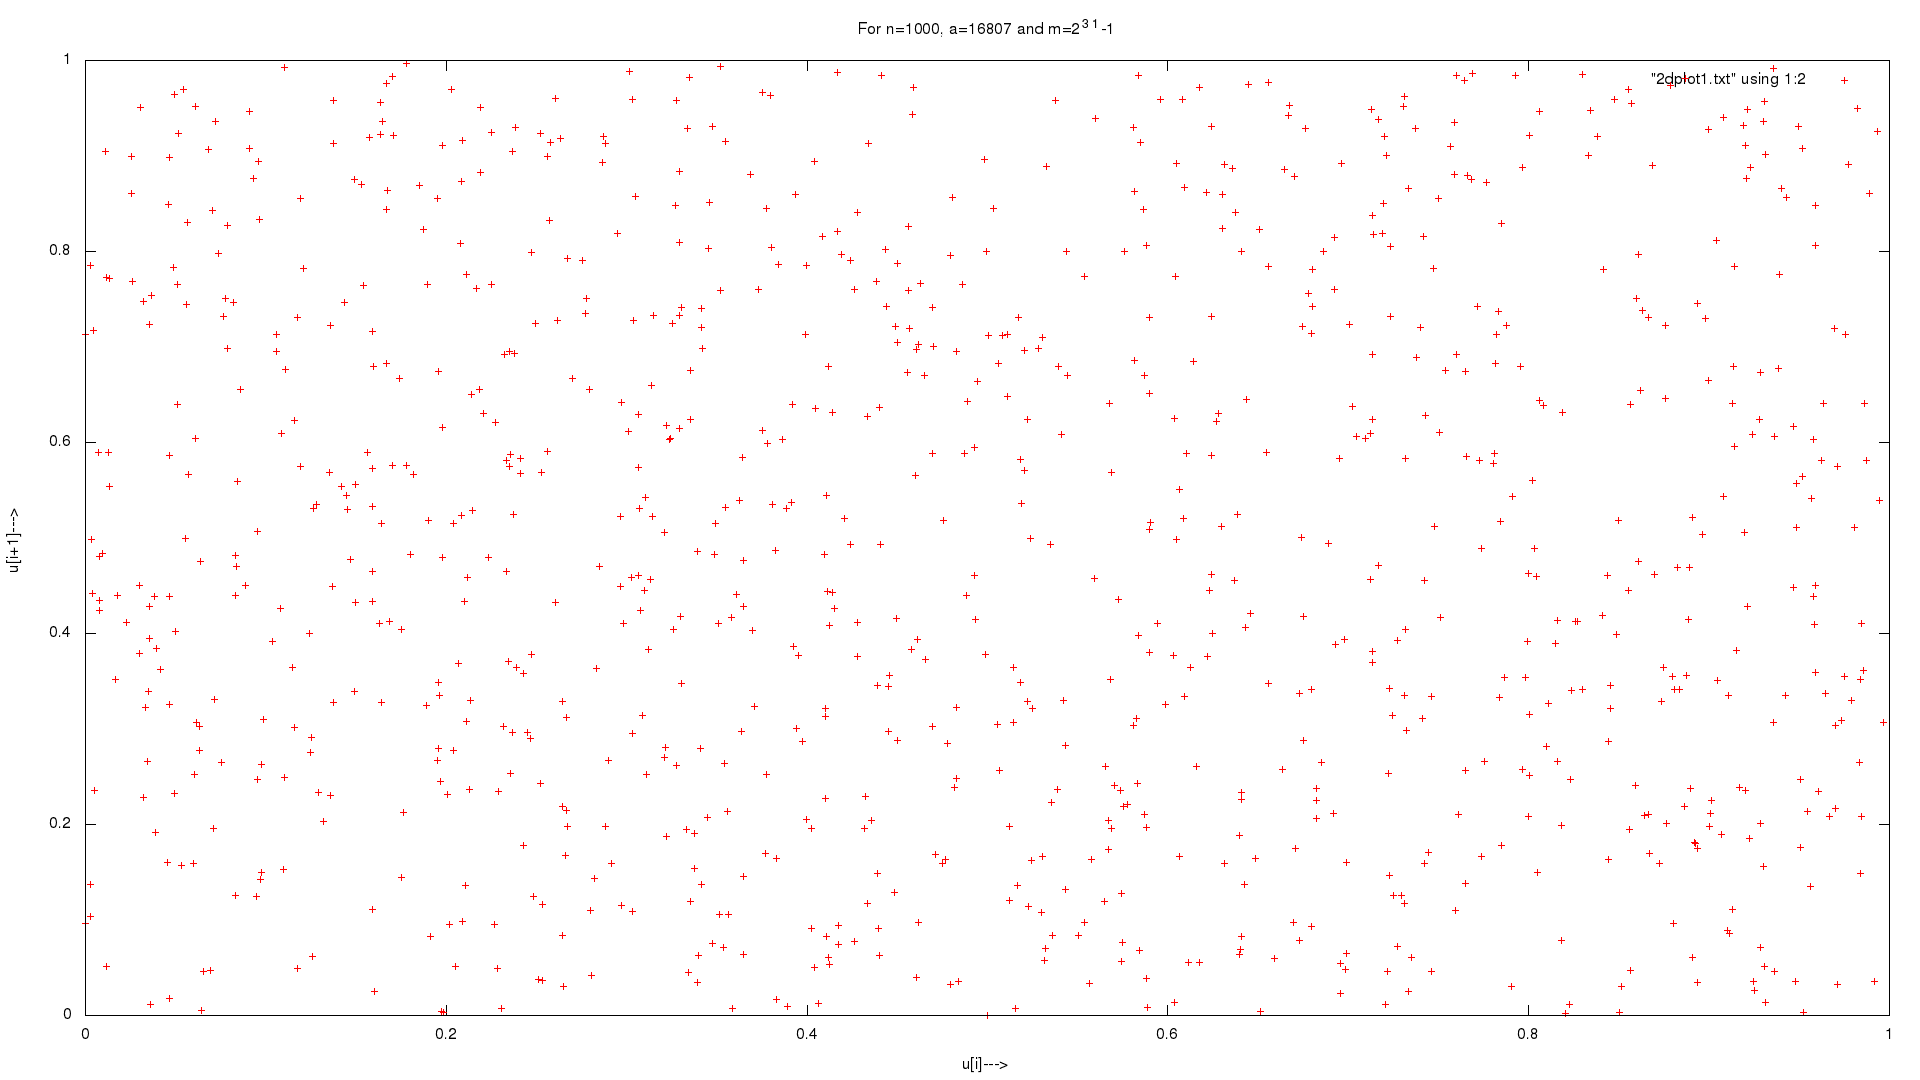
\includegraphics[width=1.0\textwidth]{q1_2d_plot1.png}}
	\caption{2D-graph of $(u_i,u_{i+1})$ for a=16807, $m=2^{31}-1$ for 1000 random numbers}
\end{figure}
\begin{figure}[H]
	\centering
	\subfloat{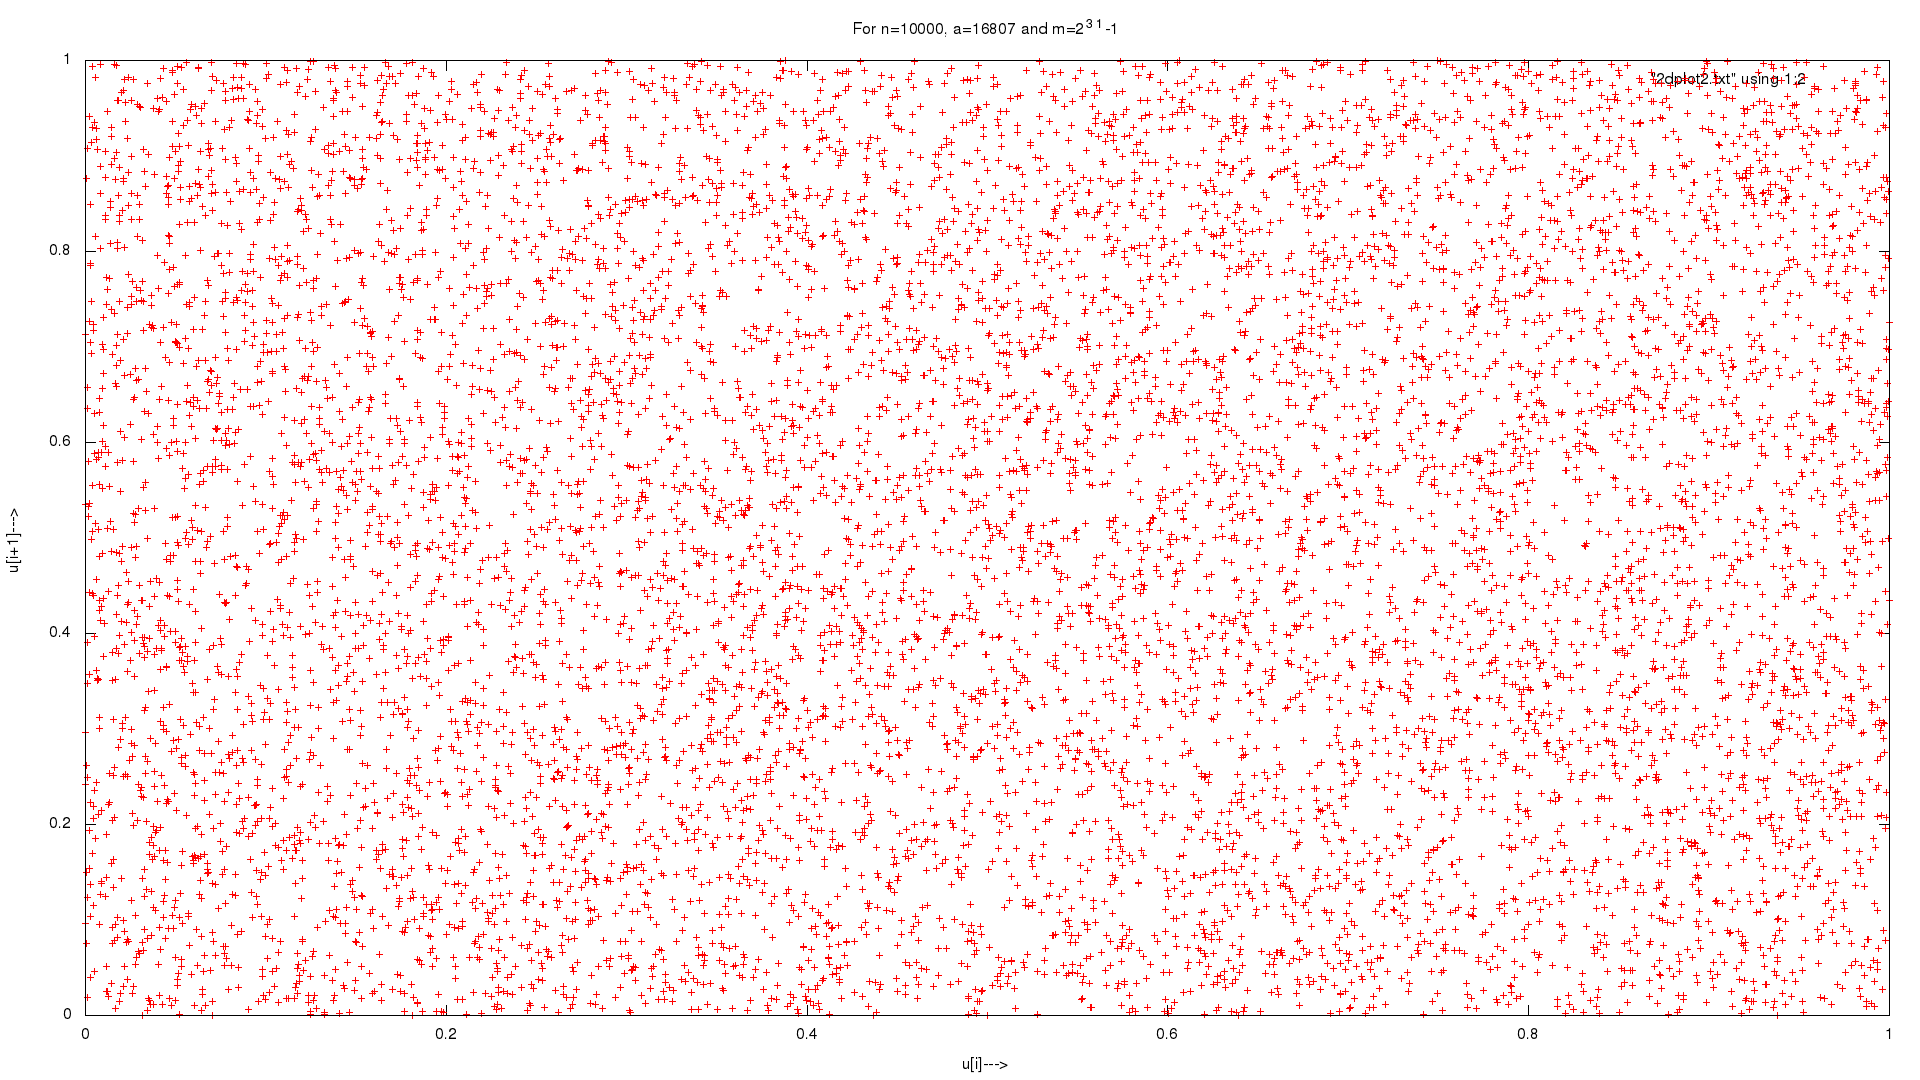
\includegraphics[width=1.0\textwidth]{q1_2d_plot2.png}}
	\caption{2D-graph of $(u_i,u_{i+1})$ for a=16807, $m=2^{31}-1$ for 10000 random numbers}
\end{figure}
\begin{figure}[H]
	\centering
	\subfloat{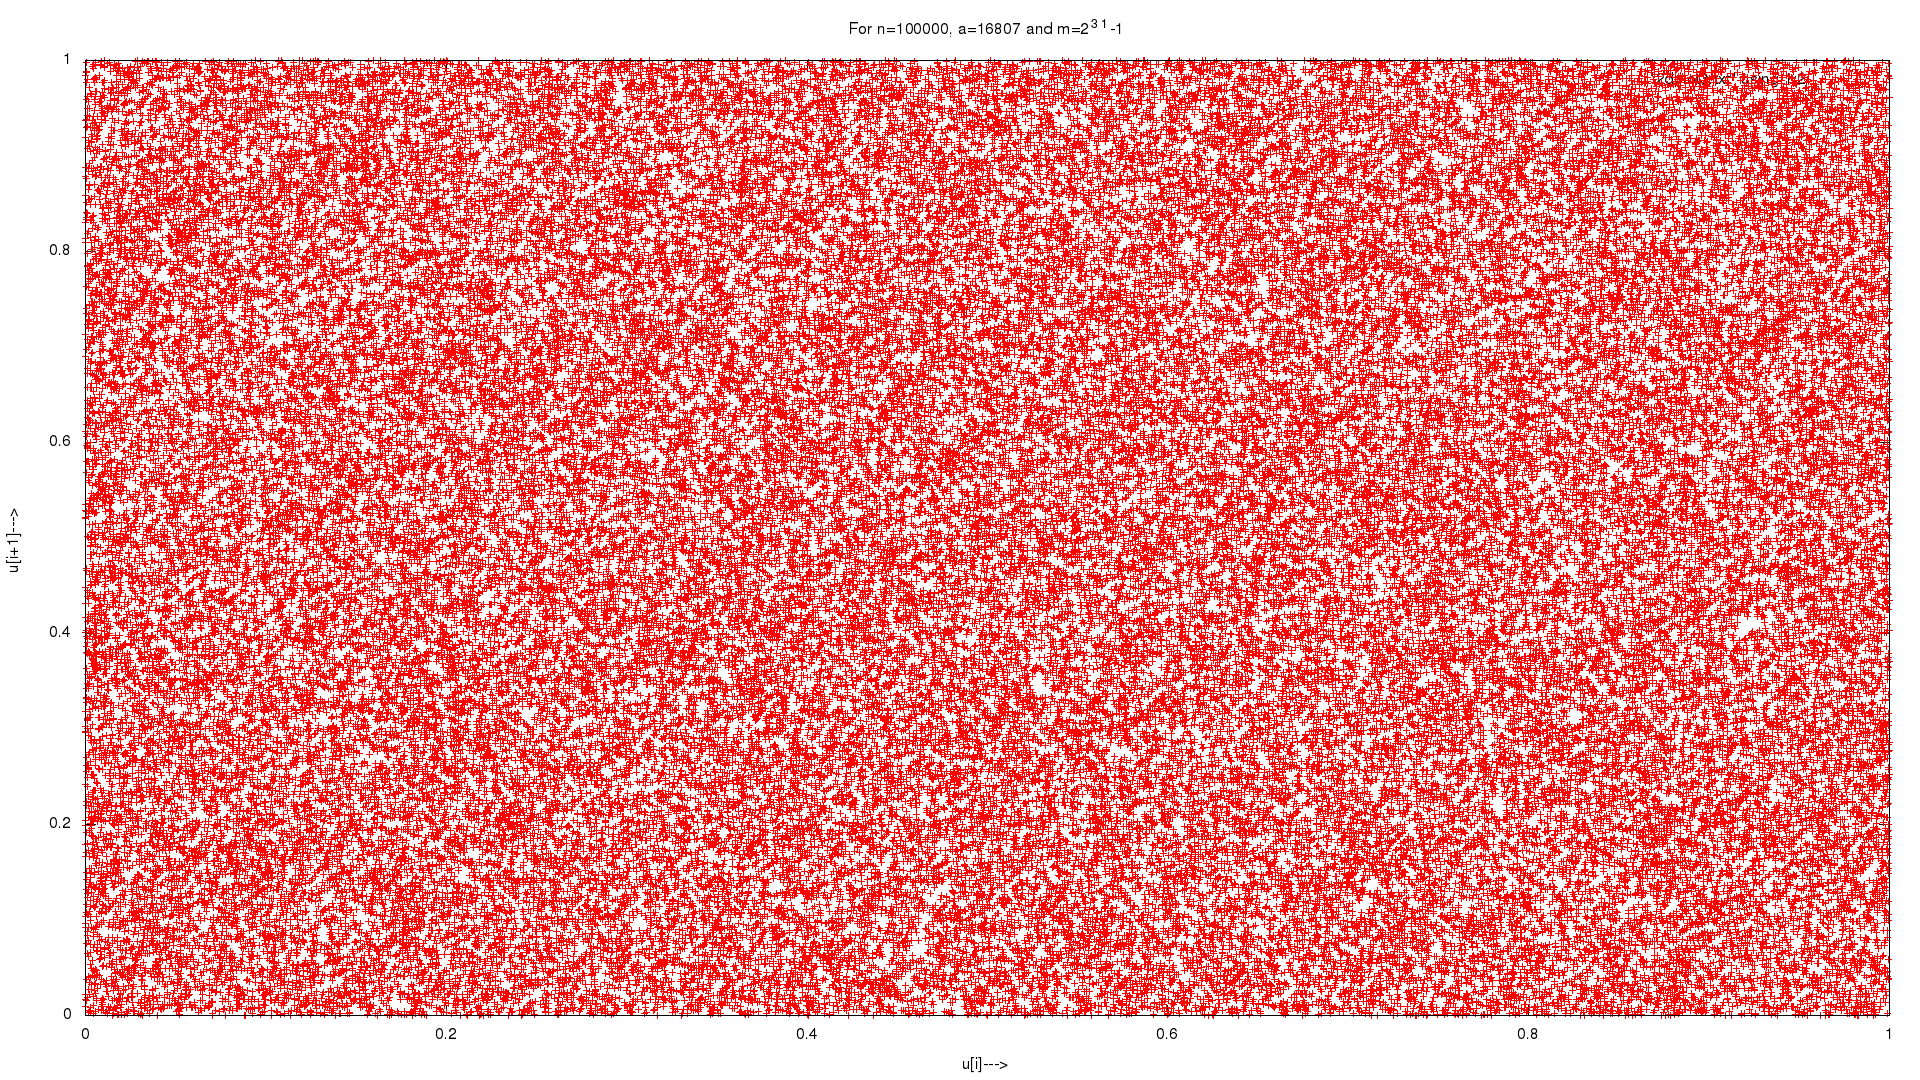
\includegraphics[width=1.0\textwidth]{q1_2d_plot3.png}}
	\caption{2D-graph of $(u_i,u_{i+1})$ for a=16807, $m=2^{31}-1$ for 100000 random numbers}
\end{figure}
\begin{figure}[H]
	\centering
	\subfloat{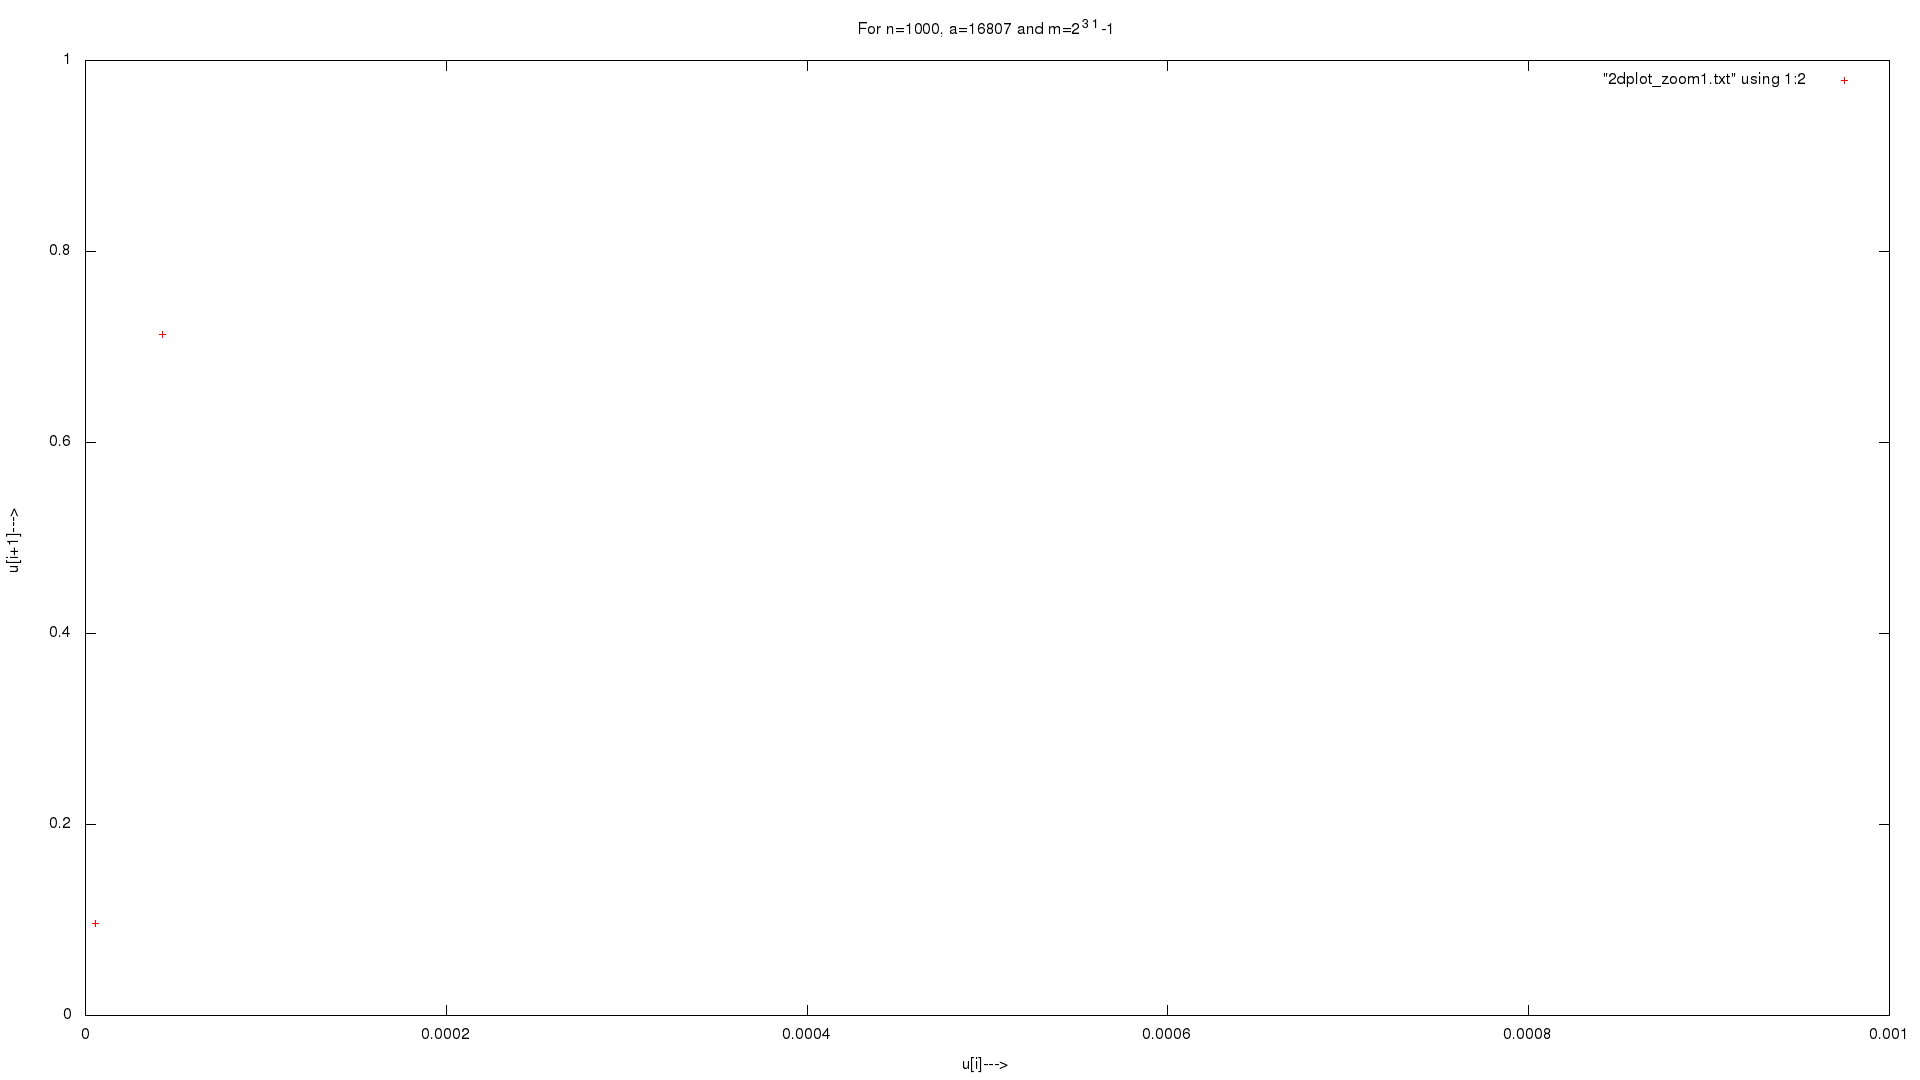
\includegraphics[width=1.0\textwidth]{q1_2d_plot_zoom1.png}}
	\caption{Zoomed $(u_i,u_{i+1})$ for a=16807, $m=2^{31}-1$ for 1000 random numbers}
\end{figure}
\begin{figure}[H]
	\centering
	\subfloat{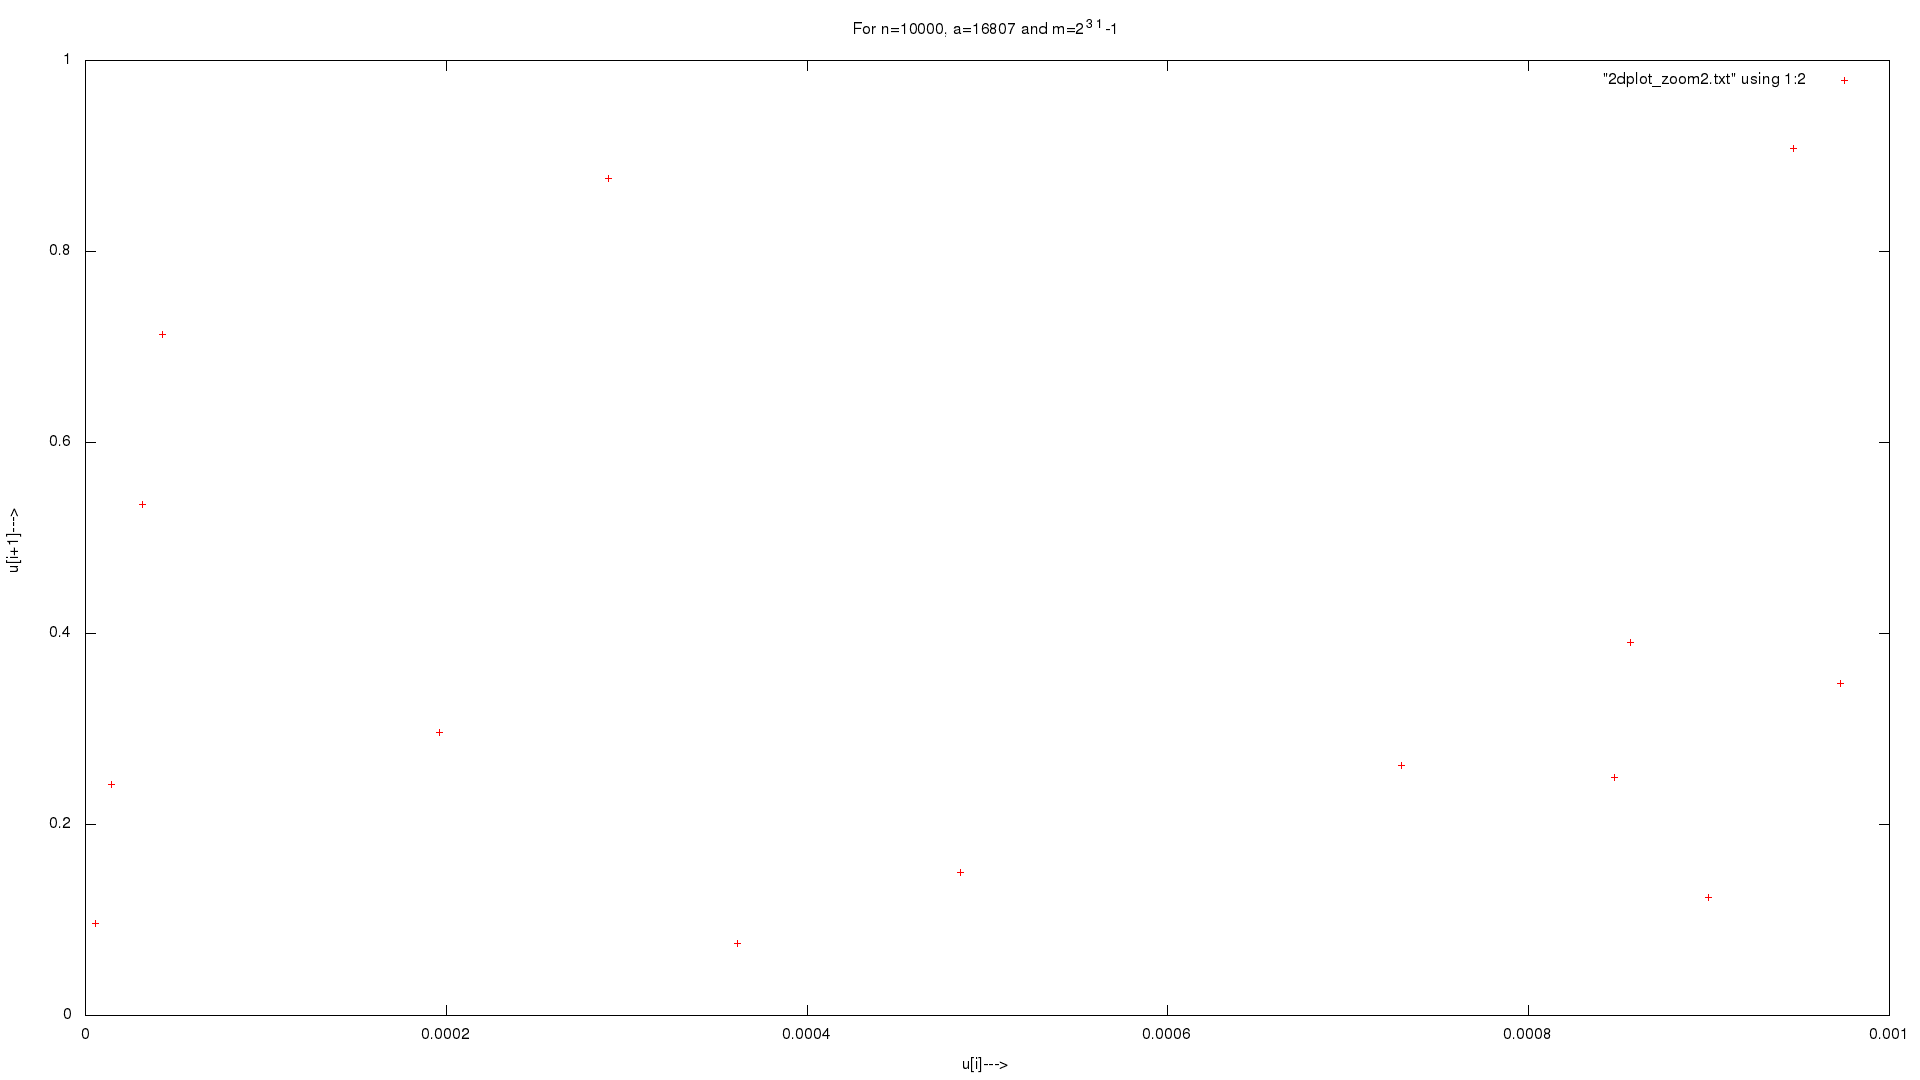
\includegraphics[width=1.0\textwidth]{q1_2d_plot_zoom2.png}}
	\caption{Zoomed $(u_i,u_{i+1})$ for a=16807, $m=2^{31}-1$ for 10000 random numbers}
\end{figure}
\begin{figure}[H]
	\centering
	\subfloat{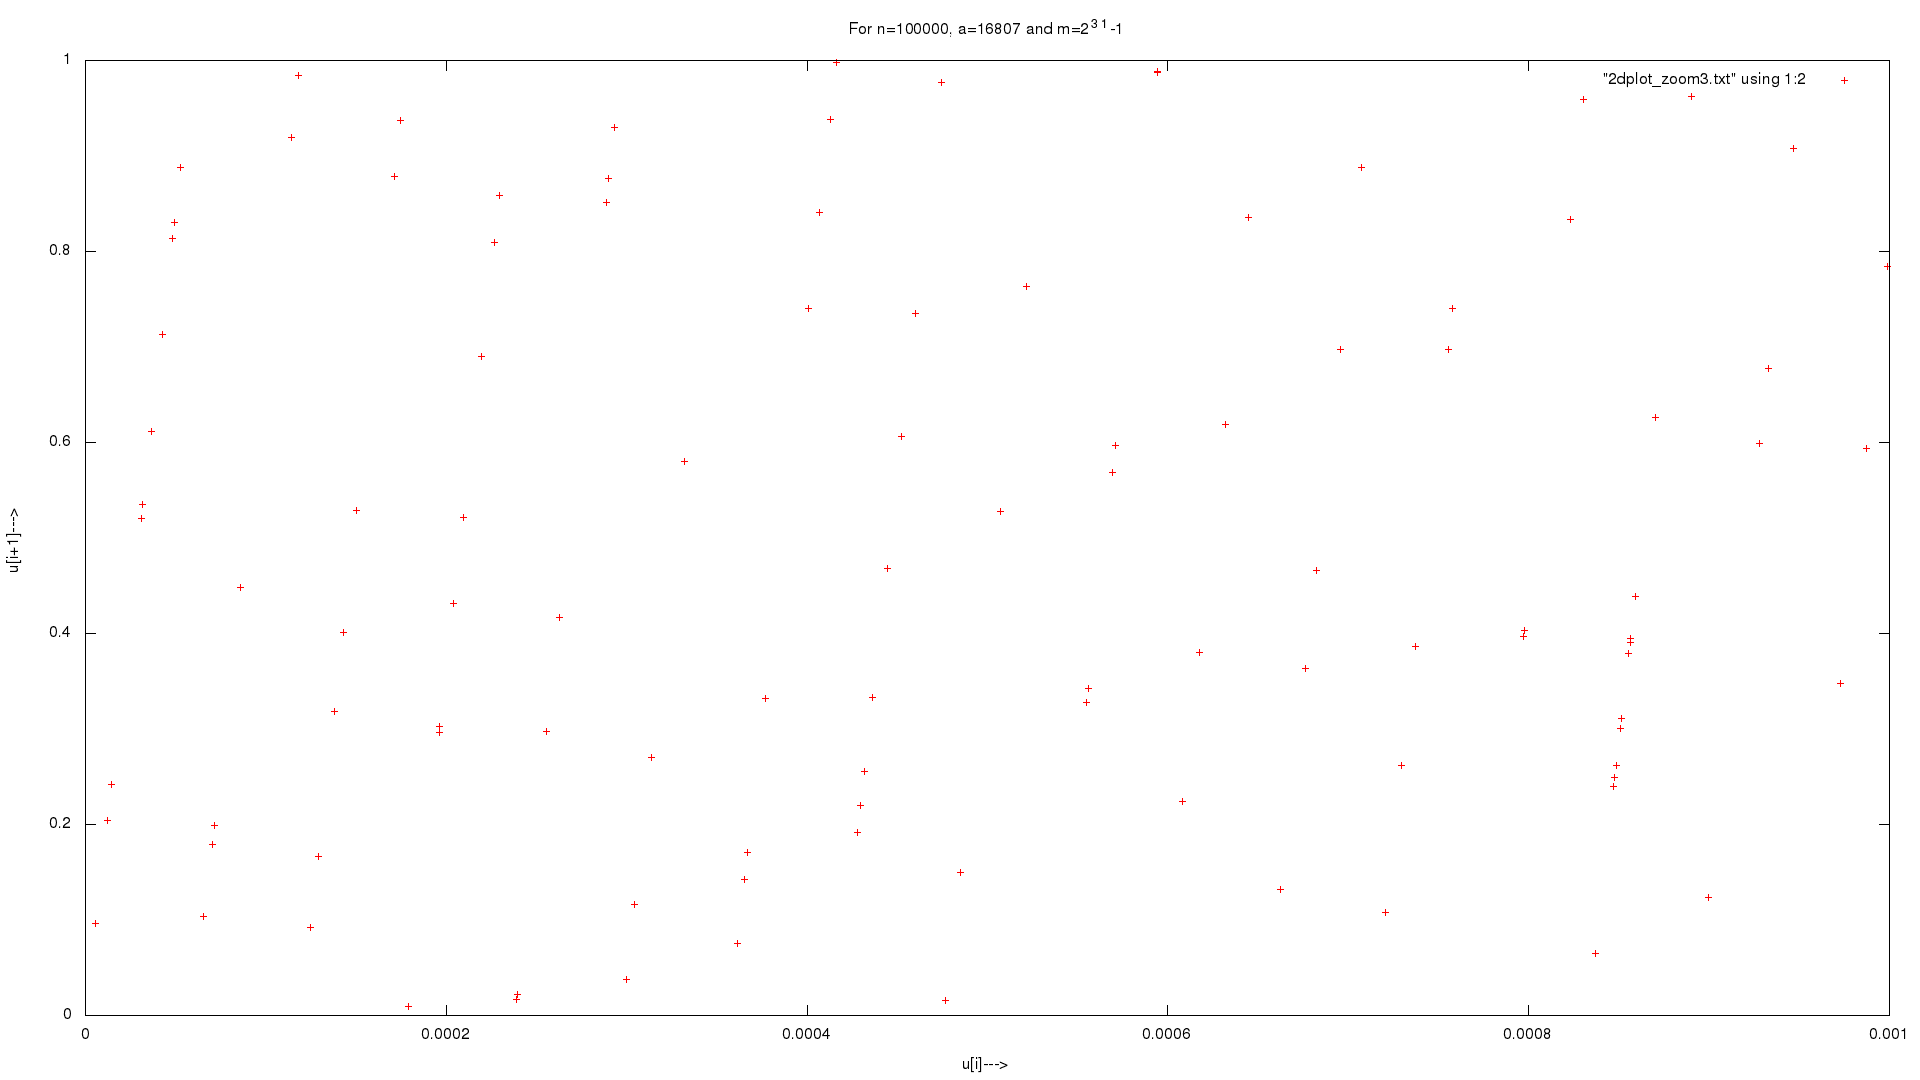
\includegraphics[width=1.0\textwidth]{q1_2d_plot_zoom3.png}}
	\caption{Zoomed $(u_i,u_{i+1})$ for a=16807, $m=2^{31}-1$ for 100000 random numbers}
\end{figure}
\newpage
\underline{Observations:}
\begin{itemize}
\item The plot of $(u_i,u_{i+1}$) got more denser and amount of white gaps in graph decrease as the number of random numbers generated are increased.
\item When $u_i$ is zoomed into the range $u_i \in [0,0.001]$, points are observed to lie on distinct parallel lines as number of random numbers generated are increased.
\item These lines are seperated by a constant distance.
\item This shows that these pseudo random numbers actually hold a correlation between them.
\end{itemize}
\newpage
\Large\textbf{{\underline{Question 2}}}\\
Consider the extended Fibonacci generator :\\
$$U_i = (U_{i-17} + U_{i-5} ) mod 2^{31}.$$
(a) Use the linear congruence generator to generate the first 17 values of $U_i$ . (b) Then generate the values of $U_i$ (say for 1000, 10000 and 100000 values). (c) For each of the above set of values plot $(U_i , U_{i+1} )$. (d) Observe (give the values) the convergence of the sample mean and sample variance towards actual values, and generate a probability distribution with, say, 1000 values generated. (e) Compute the autocorrelation of lags 1, 2, 3, 4, and 5 with 1000 generated values.\\
\Large\textbf{{\underline{Solution}}}\\\\
\underline{C++ Code:}
\begin{lstlisting}
#include <iostream>
#include <fstream>
#include <cmath>

using namespace std;
int main()
{
	ofstream myfile;
	myfile.open("output.txt");
	long long int x[3][100000];//for storing x[i]
	float u[1000];//for storing u[i]
	int f[200];
	int temp;
	long long int mean[3][100000];
	long long int var[3][100000];
	int l[6]={0,1,2,3,4,5};//amt of lag
	float autocorelation[6];

	long long int a,m;//for computing first 17 values of x[i], data taken from question 1
	int i,j;
	long long int q,r,k,b;
	x[0][0]=12345;
	x[1][0]=12345;
	x[2][0]=12345;
	
	a=16807;
	m=2147483399;
	b=pow(2,31);
	long long int n[3]={1000,10000,100000};

	//computation part

	for(i=0;i<3;i++) //loop for n[i]
	{
		for(j=0;j<16;j++) //for computing x[i][1] to x[i][16]
		{
			q=m/a;
			r=m%a;
			k=x[i][j]/q;
			x[i][j+1]=(a*(x[i][j]-(k*q)))-(k*r);
			if (x[i][j+1]<0)
				x[i][j+1]=x[i][j+1]+m;
		}
		for (j=16;j<n[i]-1;j++)
		{
			x[i][j+1]=((x[i][j-16])+(x[i][j-4]))% b;
		}

		
		//computing mean
		mean[i][0]=x[i][0];
		for(j=1;j<n[i];j++) 
		{
			mean[i][j]=((mean[i][j-1]*j)+x[i][j])/(j+1);
		}
		//computing variance
		var[i][0]=0;
		for(j=0;j<n[i]-1;j++)
		{
			var[i][j+1]=((((j+1)*(var[i][j]+pow(mean[i][j],2)))+pow(x[i][j+1],2))/(j+2))-pow(mean[i][j+1],2);
		}

		for (j=0;j<n[i];j++)
			myfile<<i<<" "<<j<<" "<<x[i][j]<<" "<<mean[i][j]<<" "<<var[i][j]<<"\n";
	}
	myfile.close();

	//computing frequency and probability distribution

	for(j=0;j<1000;j++)
	{
		u[j] = float(x[0][j])/float(b);
		temp=u[j]/0.005;
		f[temp]++;
	}

	for (j=1;j<200;j++)
		f[j]=f[j]+f[j-1];
	myfile.open("probability.txt");
	for(j=0;j<200;j++)
		myfile<<f[j]<<"\n";
	myfile.close();

	//computing autocorelation function with lags 1,2,3,4,5 

	for(i=0;i<6;i++)
	{
		for(j=l[i];j<1000;j++)
		{
			autocorelation[i]+=((float(x[0][j])-float(mean[0][999]))*(float(x[0][j-l[i]])-float(mean[0][999])));
		}
	}
	myfile.open("autocorrelation.txt");
	for(i=1;i<6;i++)
	{
		autocorelation[i]=autocorelation[i]/autocorelation[0];
		cout<<"Autocorrelation with lag "<<i<<" for 1000 random numbers = "<<autocorelation[i]<<"\n";
		myfile<<"Autocorrelation with lag "<<i<<" for 1000 random numbers = "<<autocorelation[i]<<"\n";
	}
	myfile.close();

	//printing mean to files

	myfile.open("mean1.txt");
	for (j=0;j<1000;j++)
	{
		myfile<<mean[0][j]<<"\n";
	}
	myfile.close();

	myfile.open("mean2.txt");
	for (j=0;j<10000;j++)
	{
		myfile<<mean[1][j]<<"\n";
	}
	myfile.close();

	myfile.open("mean3.txt");
	for (j=0;j<100000;j++)
	{
		myfile<<mean[2][j]<<"\n";
	}
	myfile.close();

	//printing variance to files

	myfile.open("var1.txt");
	for (j=0;j<1000;j++)
	{
		myfile<<var[0][j]<<"\n";
	}
	myfile.close();

	myfile.open("var2.txt");
	for (j=0;j<10000;j++)
	{
		myfile<<var[1][j]<<"\n";
	}
	myfile.close();

	myfile.open("var3.txt");
	for (j=0;j<100000;j++)
	{
		myfile<<var[2][j]<<"\n";
	}
	myfile.close();


	//printing plot values to files

	myfile.open("2d_plot1.txt");
	for(i=0;i<999;i++)
	{
		myfile<<x[0][i]<<"	"<<x[0][i+1]<<"\n";
	}
	myfile.close();

	myfile.open("2d_plot2.txt");
	for(i=0;i<9999;i++)
	{
		myfile<<x[1][i]<<"	"<<x[1][i+1]<<"\n";
	}
	myfile.close();

	myfile.open("2d_plot3.txt");
	for(i=0;i<99999;i++)
	{
		myfile<<x[2][i]<<"	"<<x[2][i+1]<<"\n";
	}
	myfile.close();
}
\end{lstlisting}
\underline{Output:}
\begin{lstlisting}
Autocorrelation with lag 1 for 1000 random numbers = 0.00861274
Autocorrelation with lag 2 for 1000 random numbers = -0.040237
Autocorrelation with lag 3 for 1000 random numbers = 0.0289122
Autocorrelation with lag 4 for 1000 random numbers = -0.00226832
Autocorrelation with lag 5 for 1000 random numbers = -0.0380737
\end{lstlisting}
\underline{Observations:}\\
\begin{itemize}
\item A low value of autocorrelation shows that the distribution of random numbers is quite uniform.
\item Here, an autocorrelation value of 0.0289 shows that the random numbers are quite uniformly distributed, but thisn distribution could have been more uniform for some other values of the parameters of the random number generator.
\end{itemize}
\newpage
\underline{Graphs:}
\begin{figure}[H]
	\centering
	\subfloat{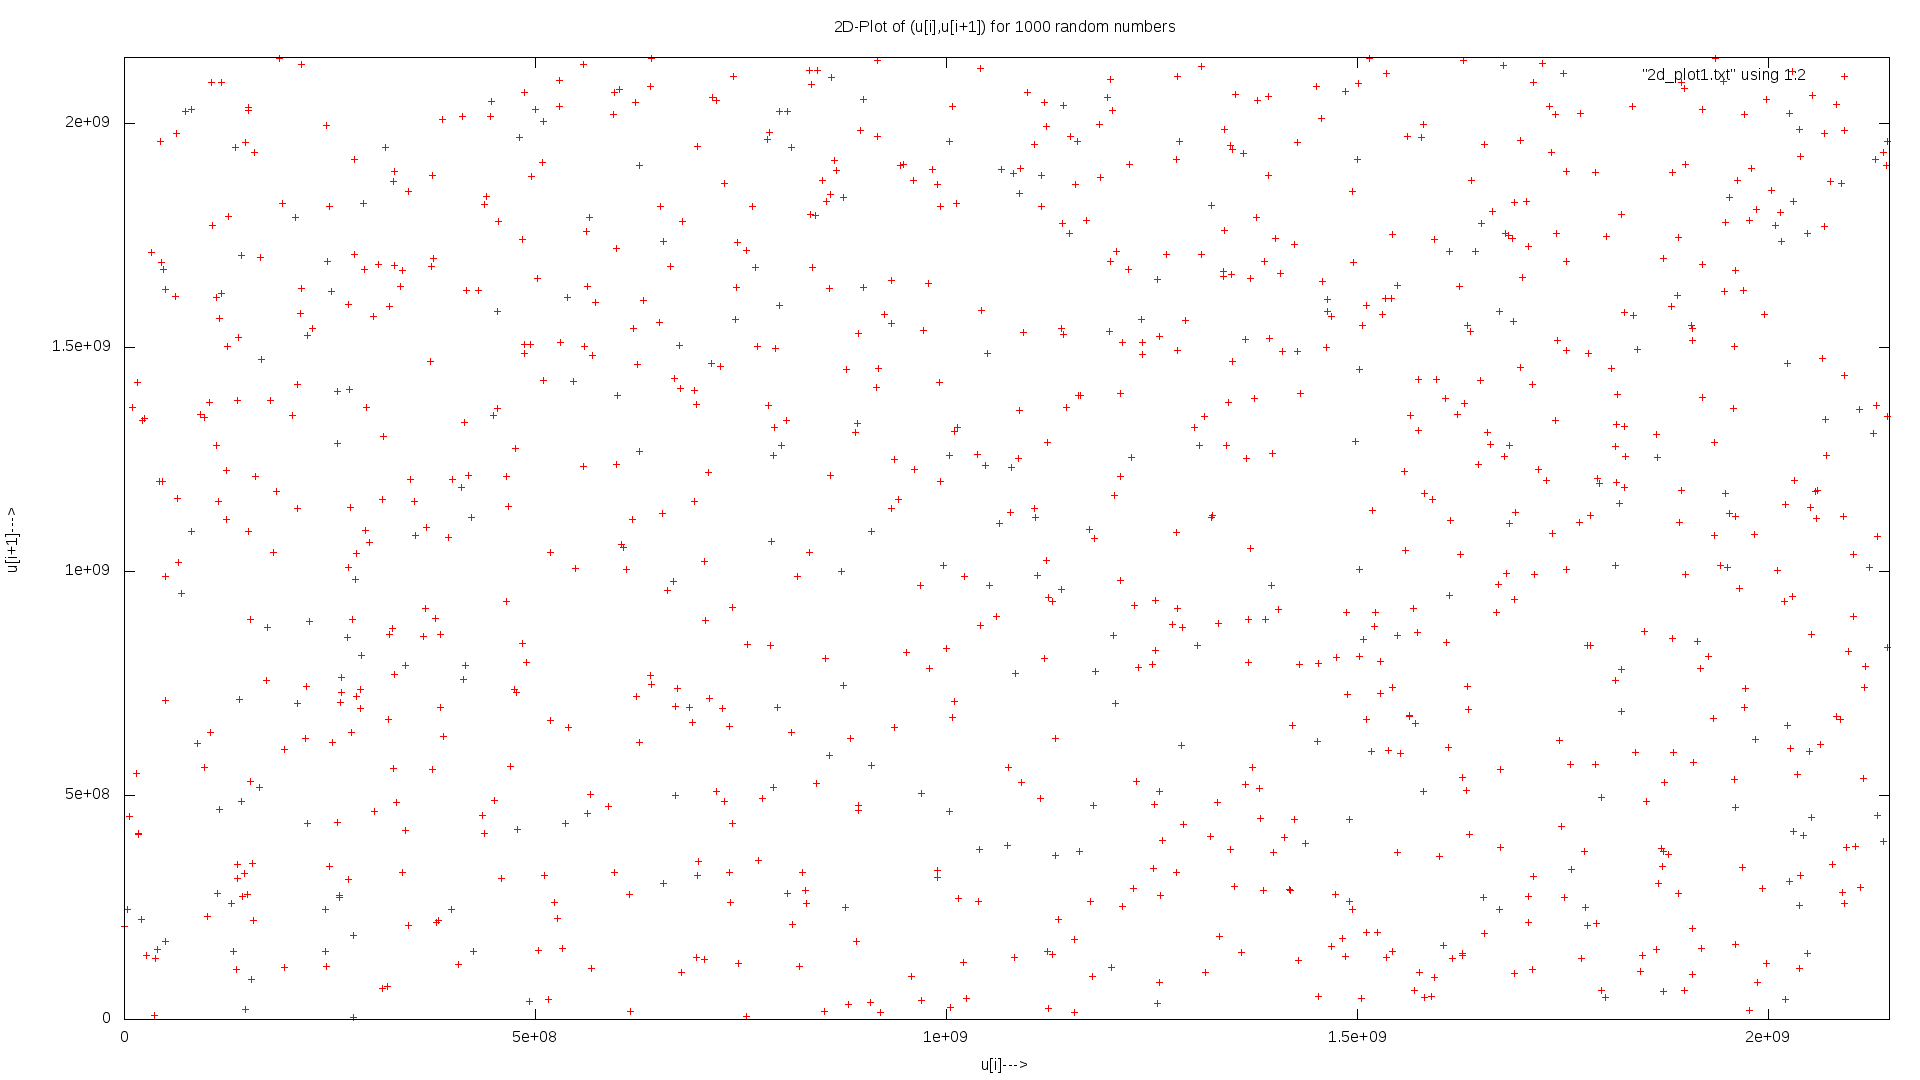
\includegraphics[width=0.9\textwidth]{q2_graph1.png}}
	\caption{2D-graph of $(u_i,u_{i+1})$ for 1000 random numbers}
\end{figure}
\begin{figure}[H]
	\centering
	\subfloat{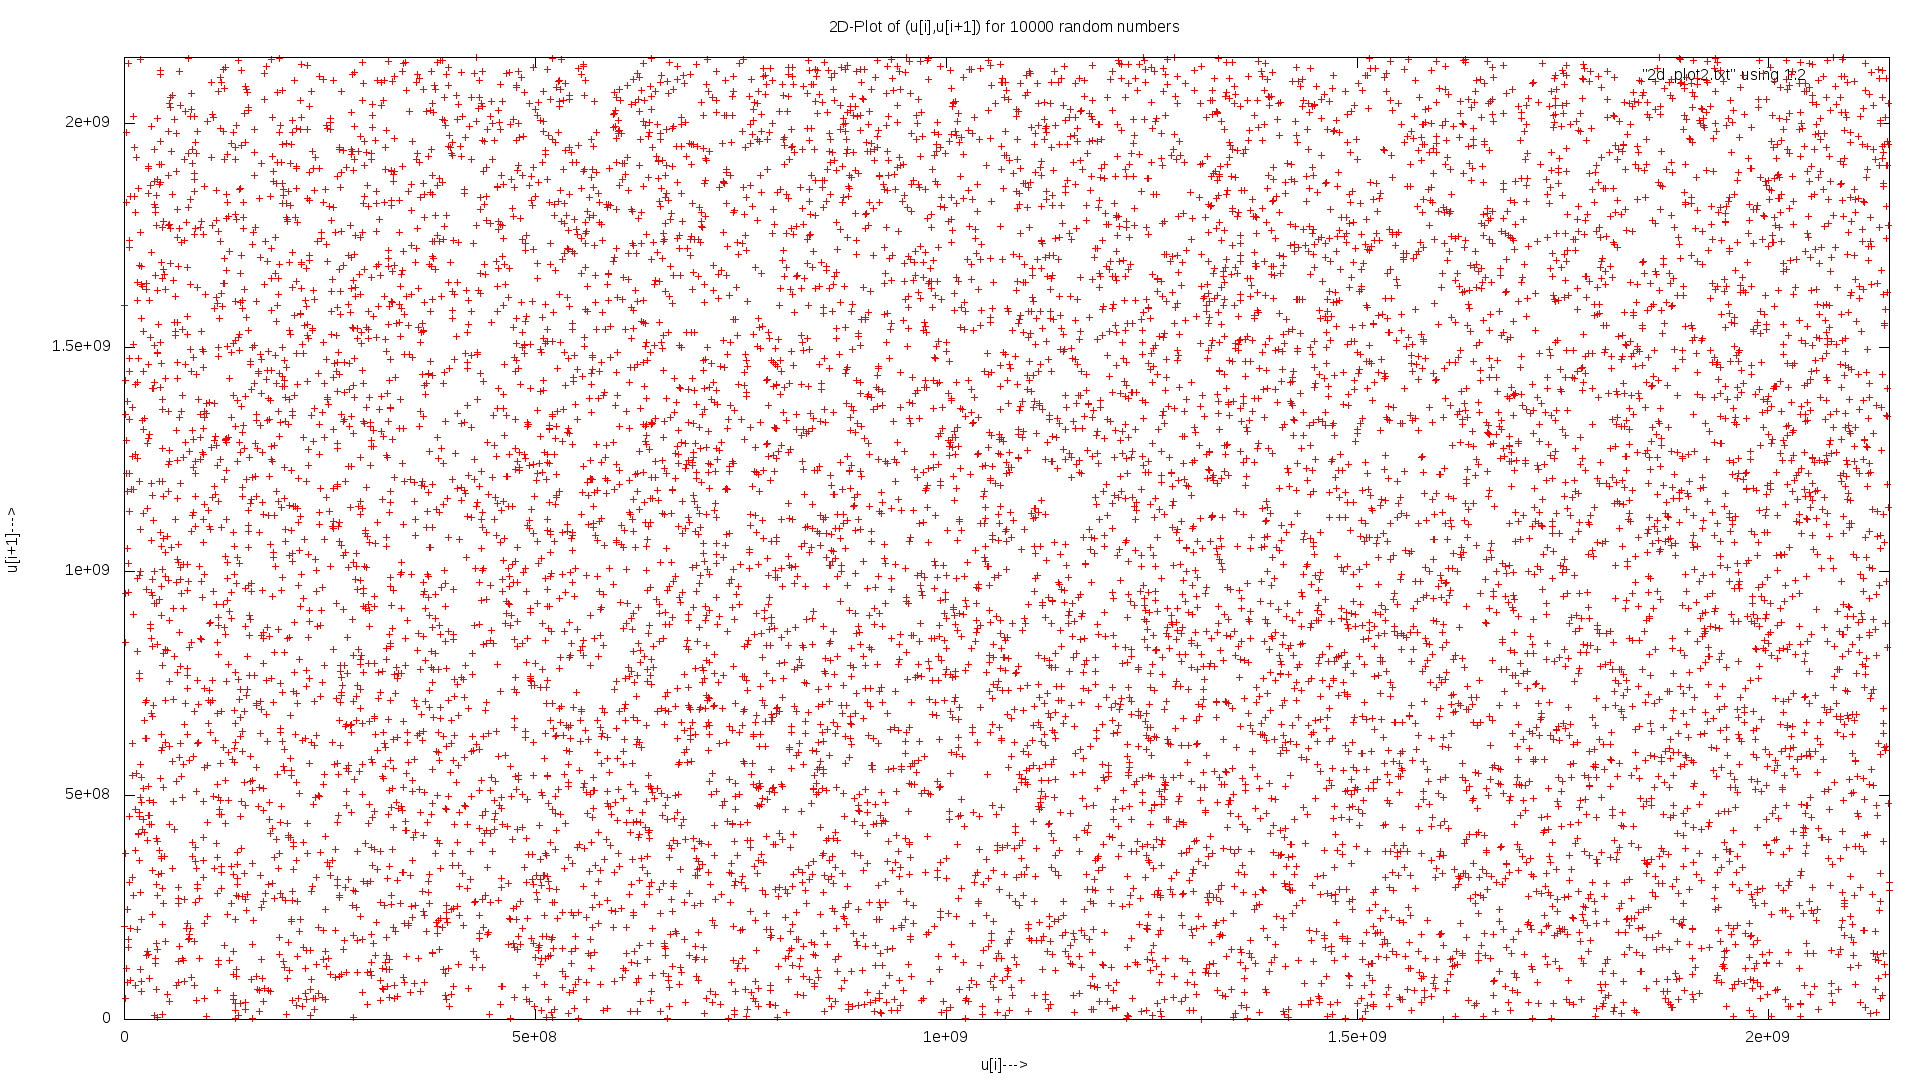
\includegraphics[width=1.0\textwidth]{q2_graph2.png}}
	\caption{2D-graph of $(u_i,u_{i+1})$ for 10000 random numbers}
\end{figure}
\begin{figure}[H]
	\centering
	\subfloat{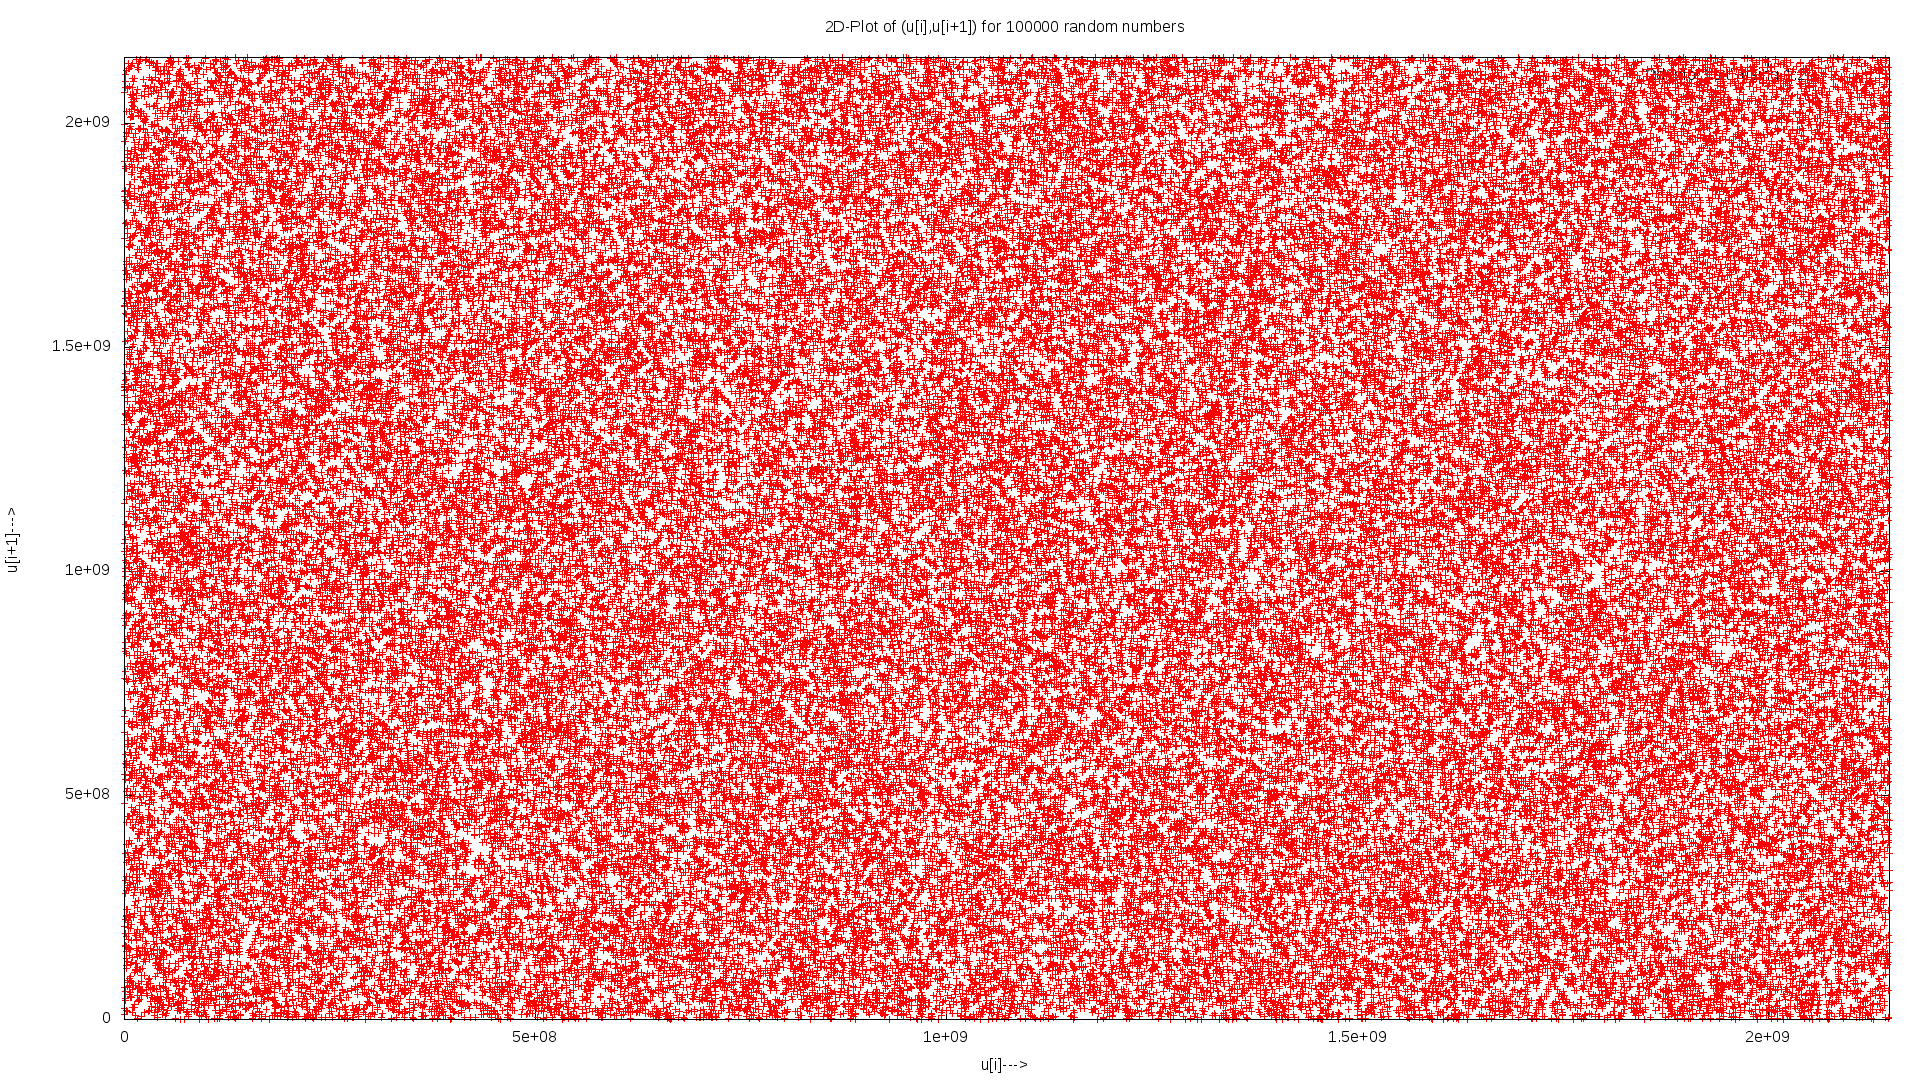
\includegraphics[width=1.0\textwidth]{q2_graph3.png}}
	\caption{2D-graph of $(u_i,u_{i+1})$ for 100000 random numbers}
\end{figure}
\begin{figure}[H]
	\centering
	\subfloat{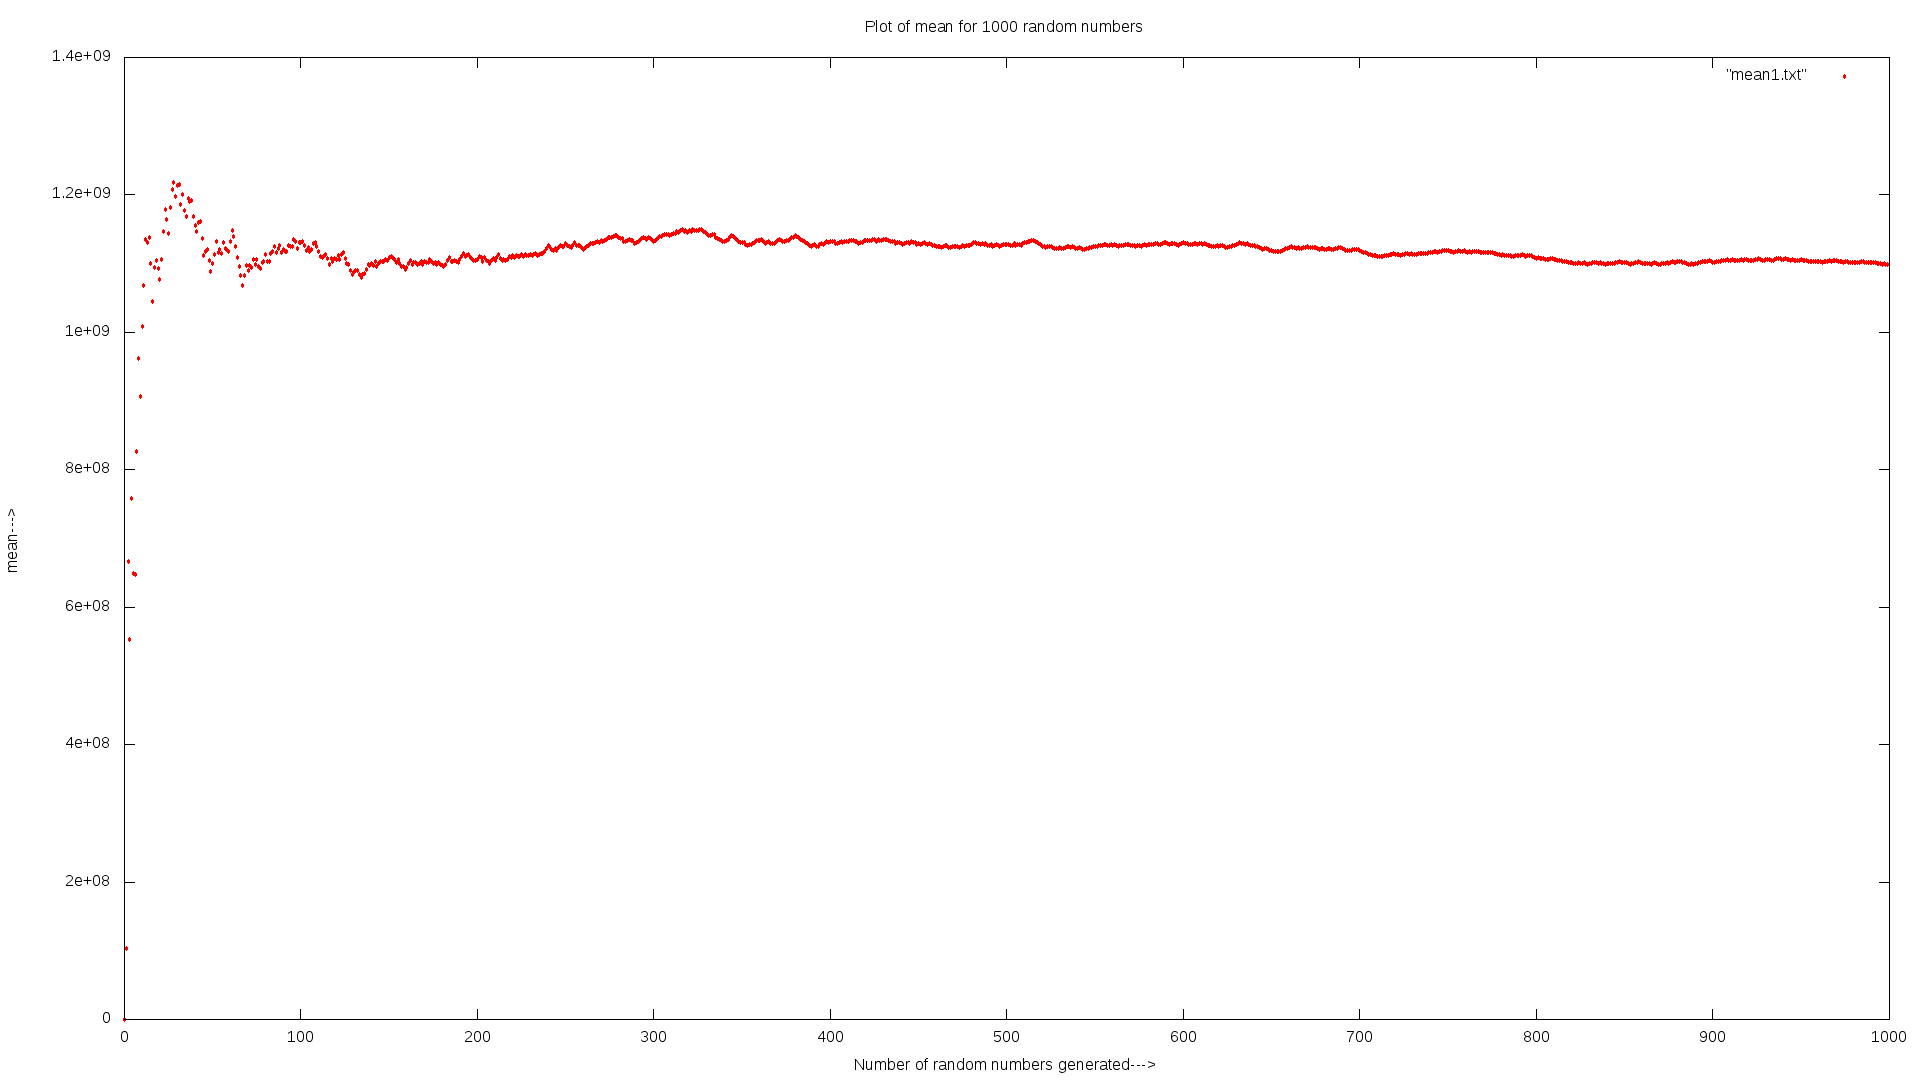
\includegraphics[width=1.0\textwidth]{q2_mean1.png}}
	\caption{Mean for 1000 random numbers}
\end{figure}
\begin{figure}[H]
	\centering
	\subfloat{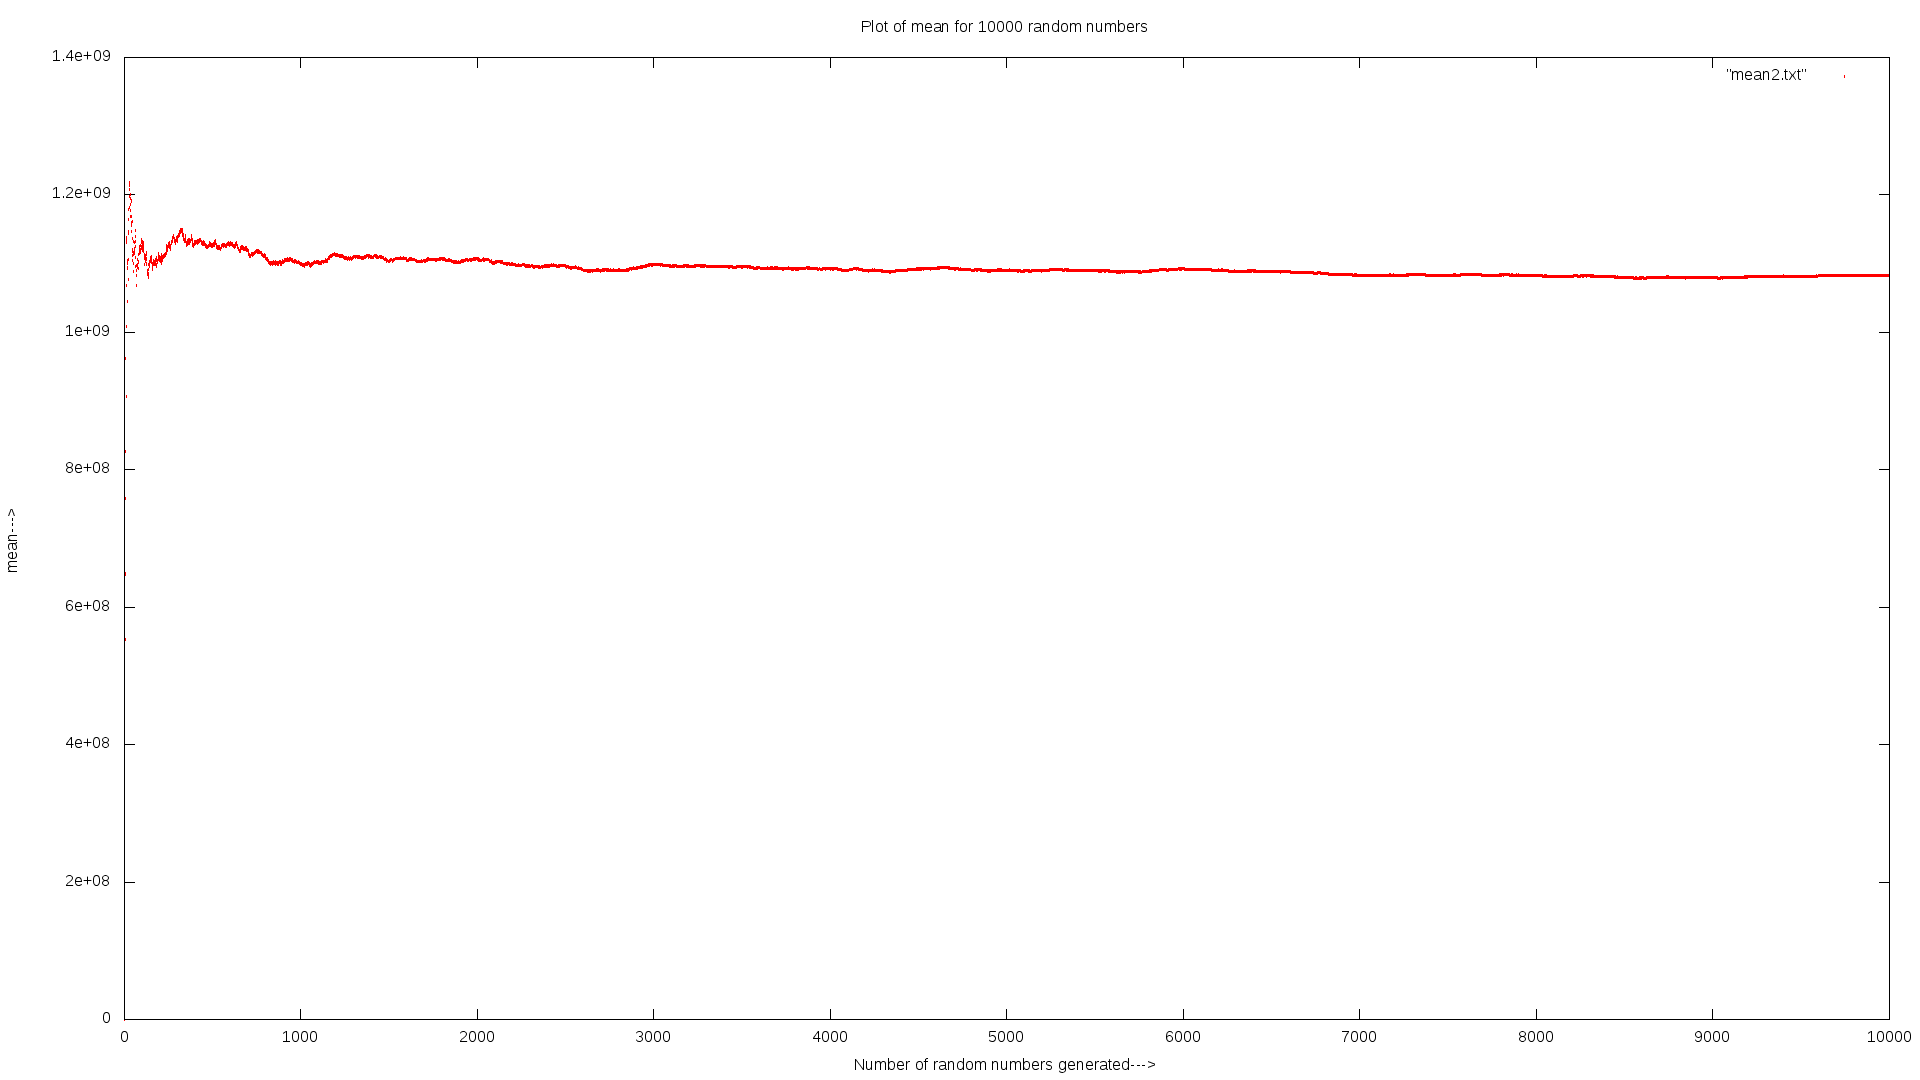
\includegraphics[width=1.0\textwidth]{q2_mean2.png}}
	\caption{Mean for 10000 random numbers}
\end{figure}
\begin{figure}[H]
	\centering
	\subfloat{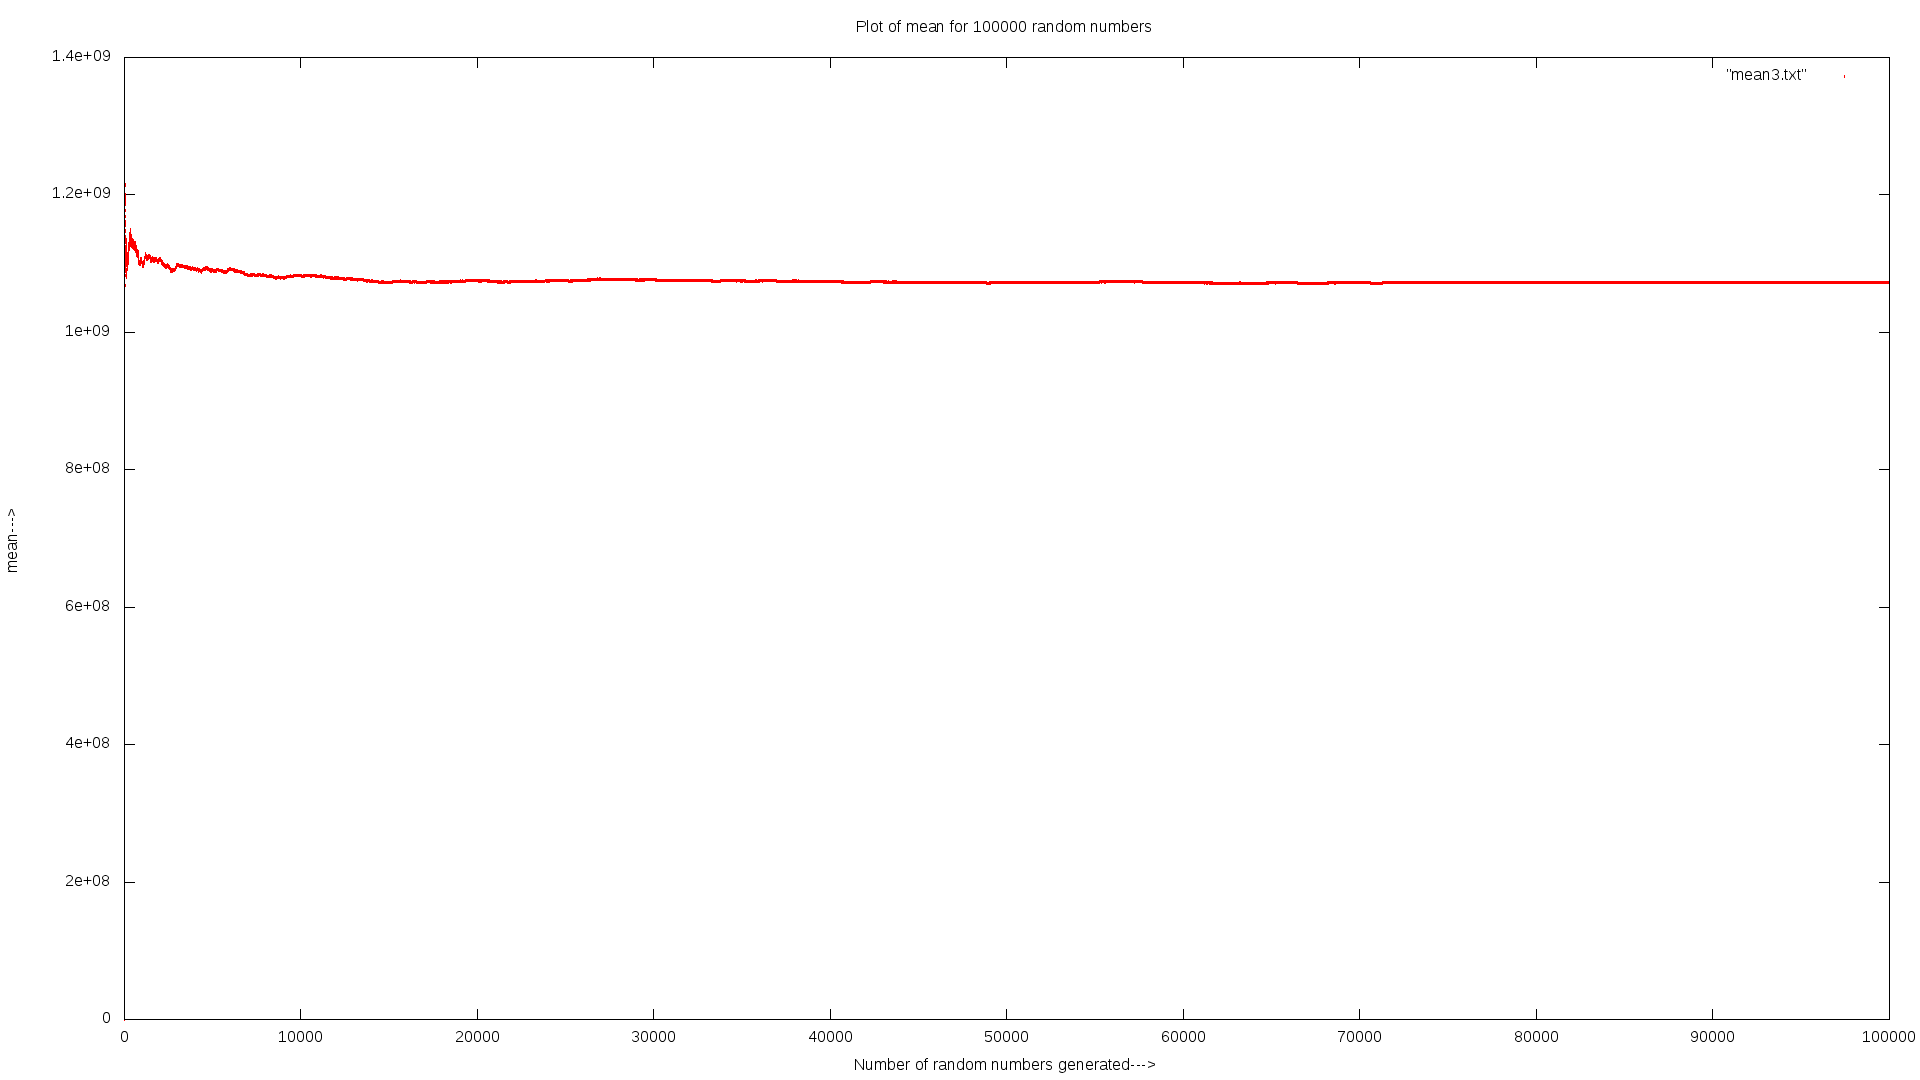
\includegraphics[width=1.0\textwidth]{q2_mean3.png}}
	\caption{Mean for 100000 random numbers}
\end{figure}
\begin{figure}[H]
	\centering
	\subfloat{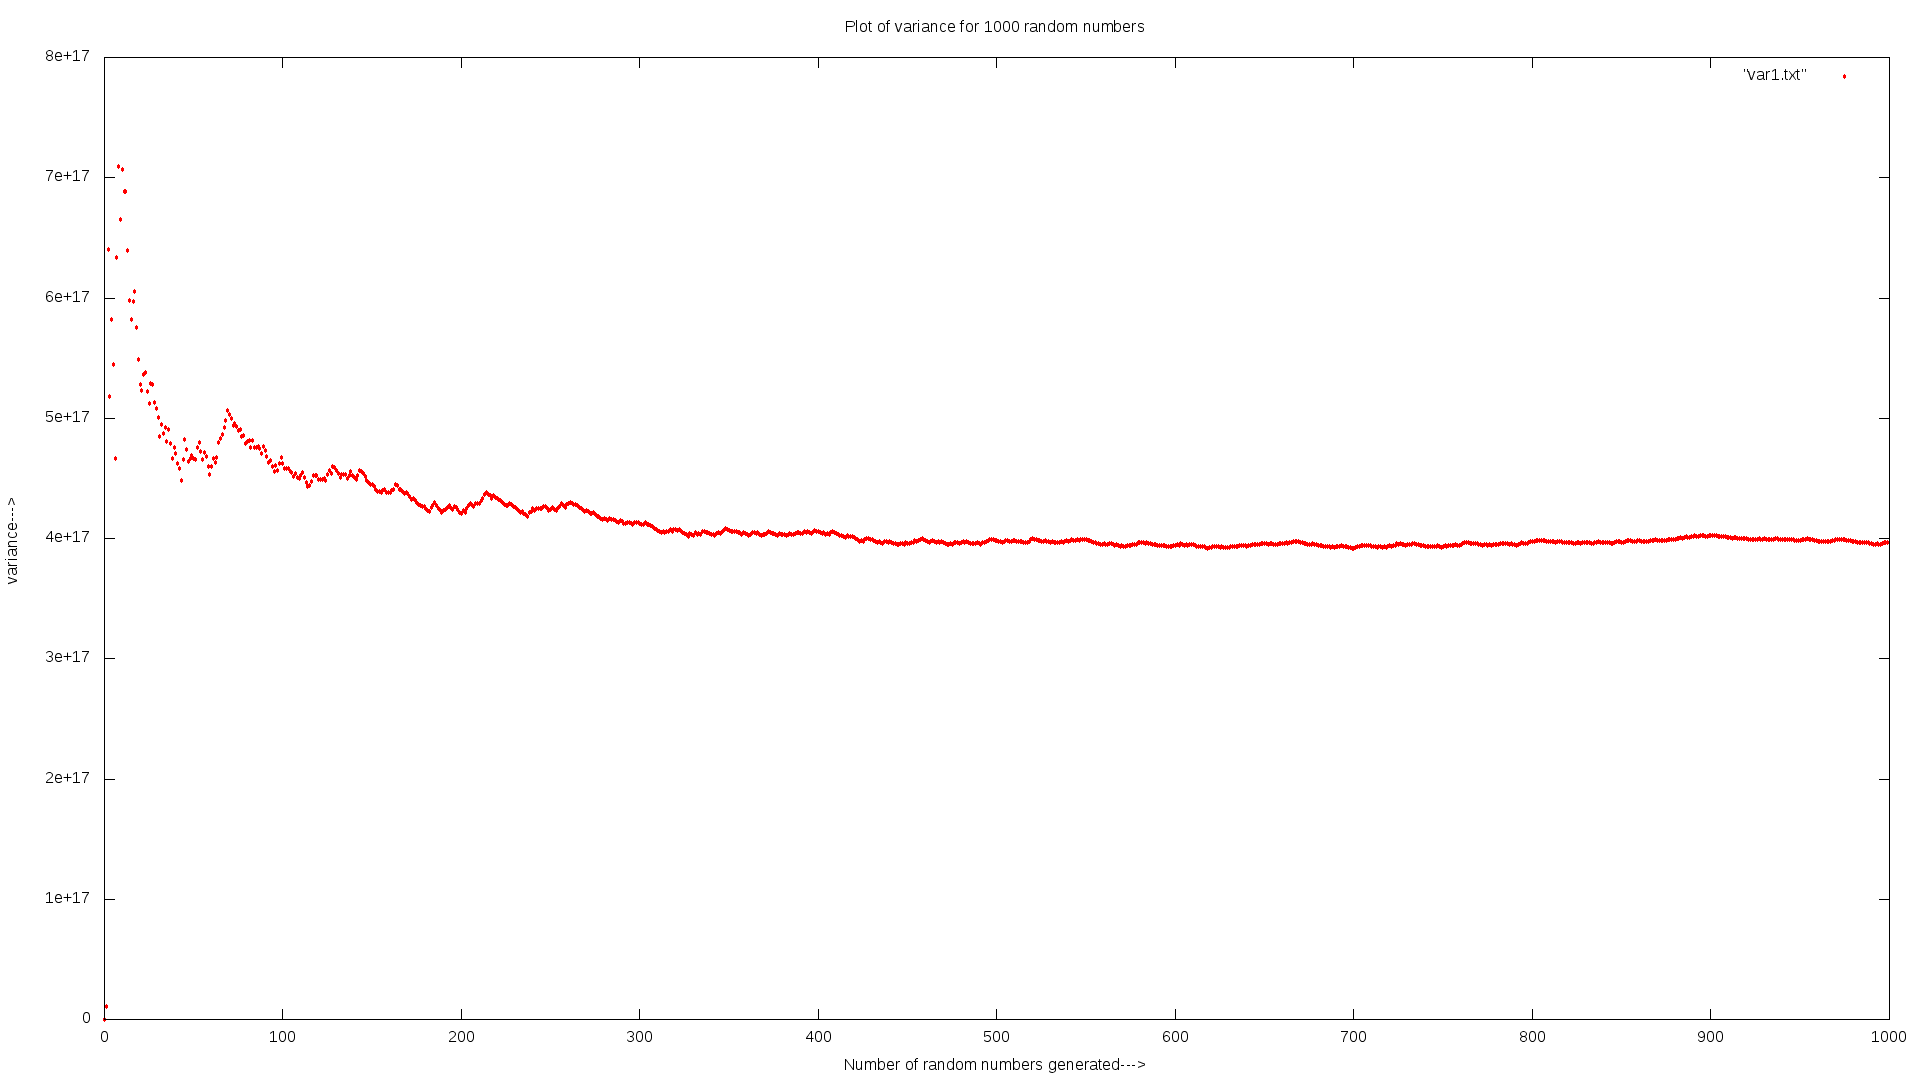
\includegraphics[width=1.0\textwidth]{q2_var1.png}}
	\caption{Variance for 1000 random numbers}
\end{figure}
\begin{figure}[H]
	\centering
	\subfloat{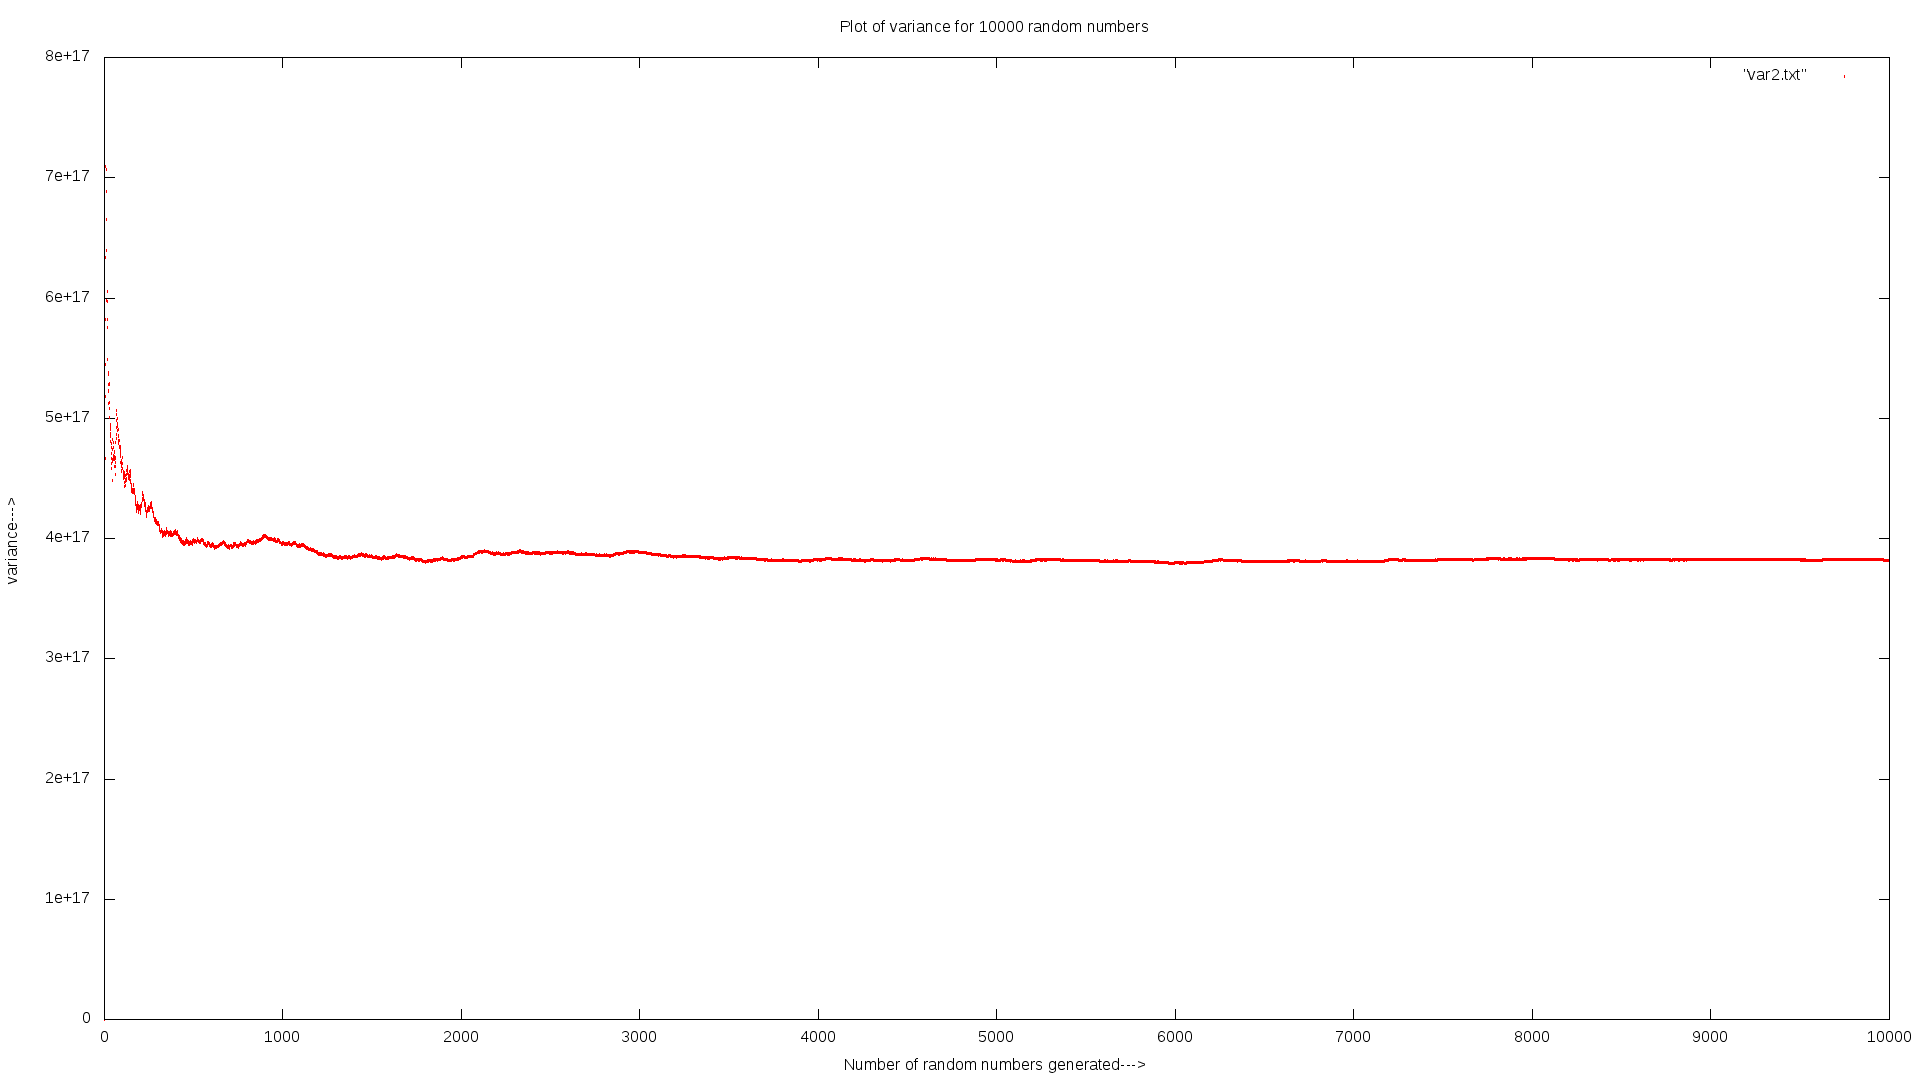
\includegraphics[width=1.0\textwidth]{q2_var2.png}}
	\caption{Variance for 10000 random numbers}
\end{figure}
\begin{figure}[H]
	\centering
	\subfloat{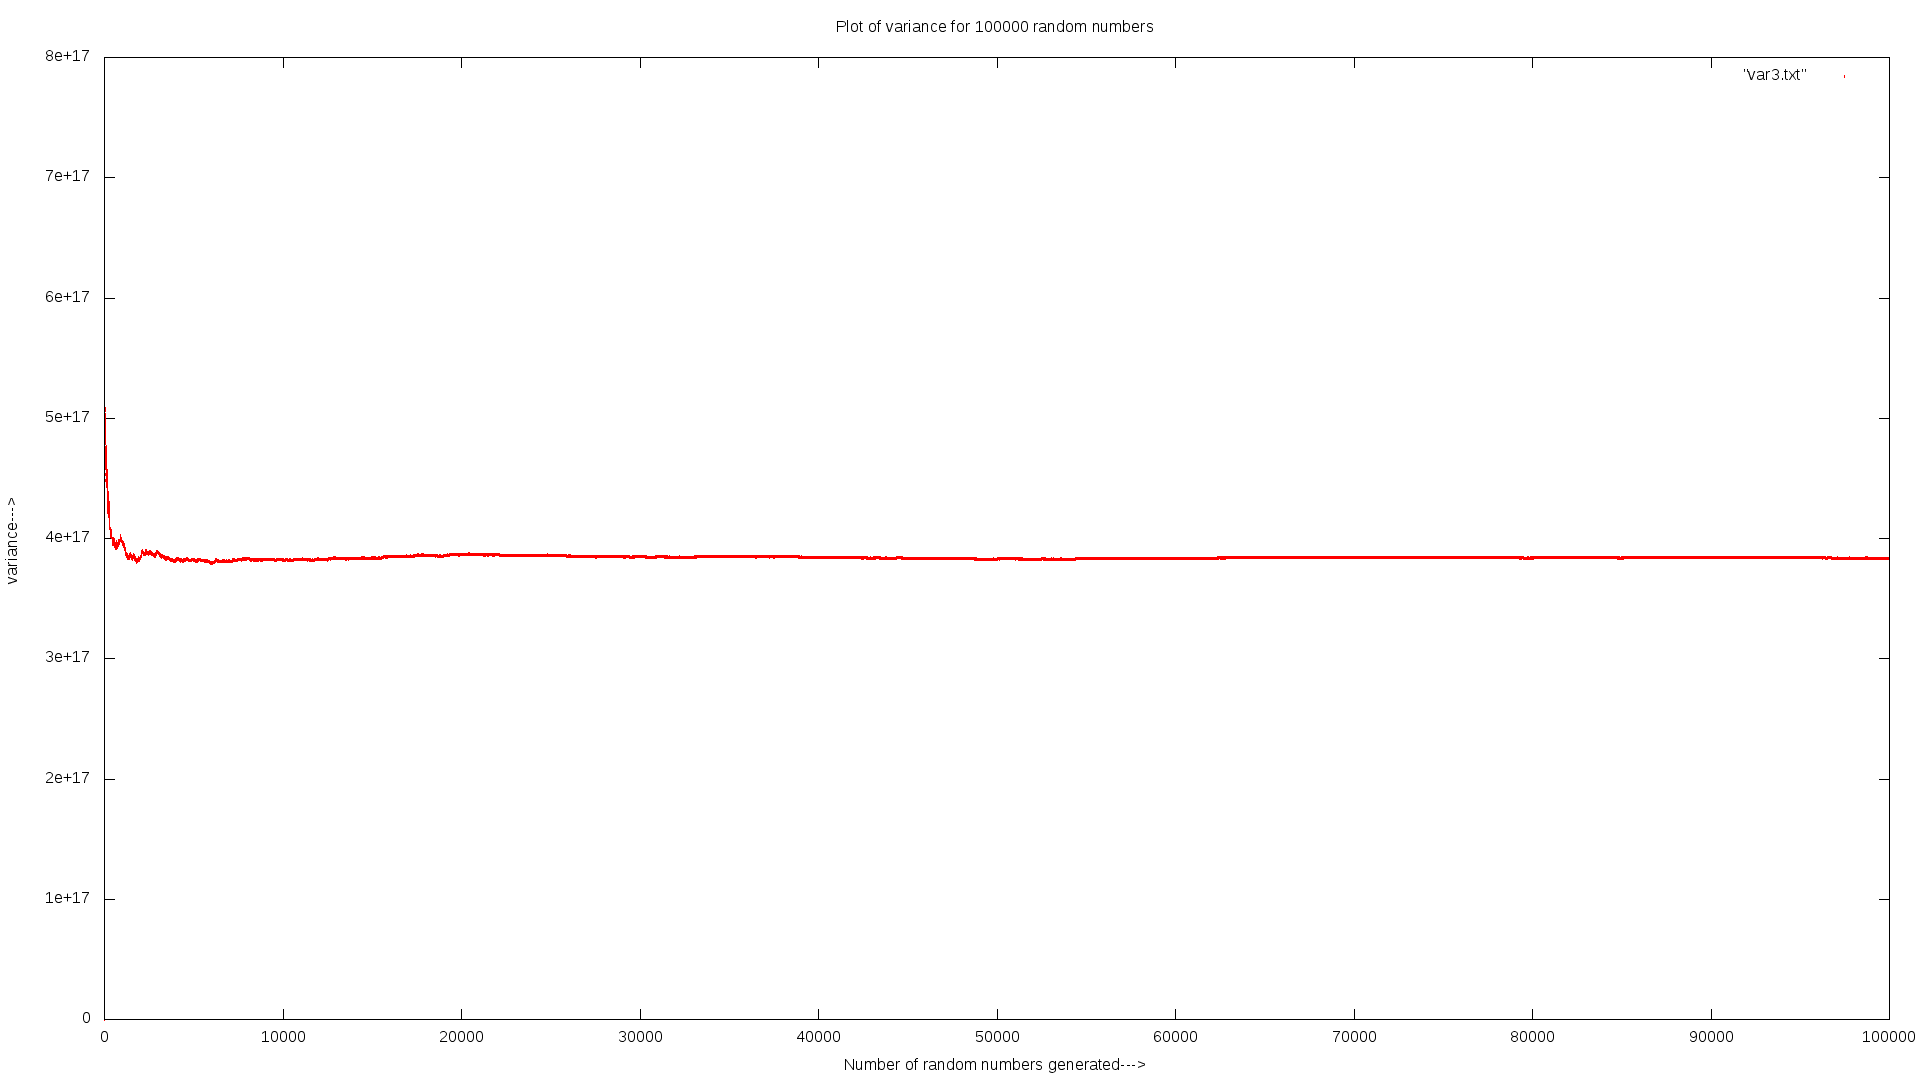
\includegraphics[width=1.0\textwidth]{q2_var3.png}}
	\caption{Variance for 100000 random numbers}
\end{figure}
\begin{figure}[H]
	\centering
	\subfloat{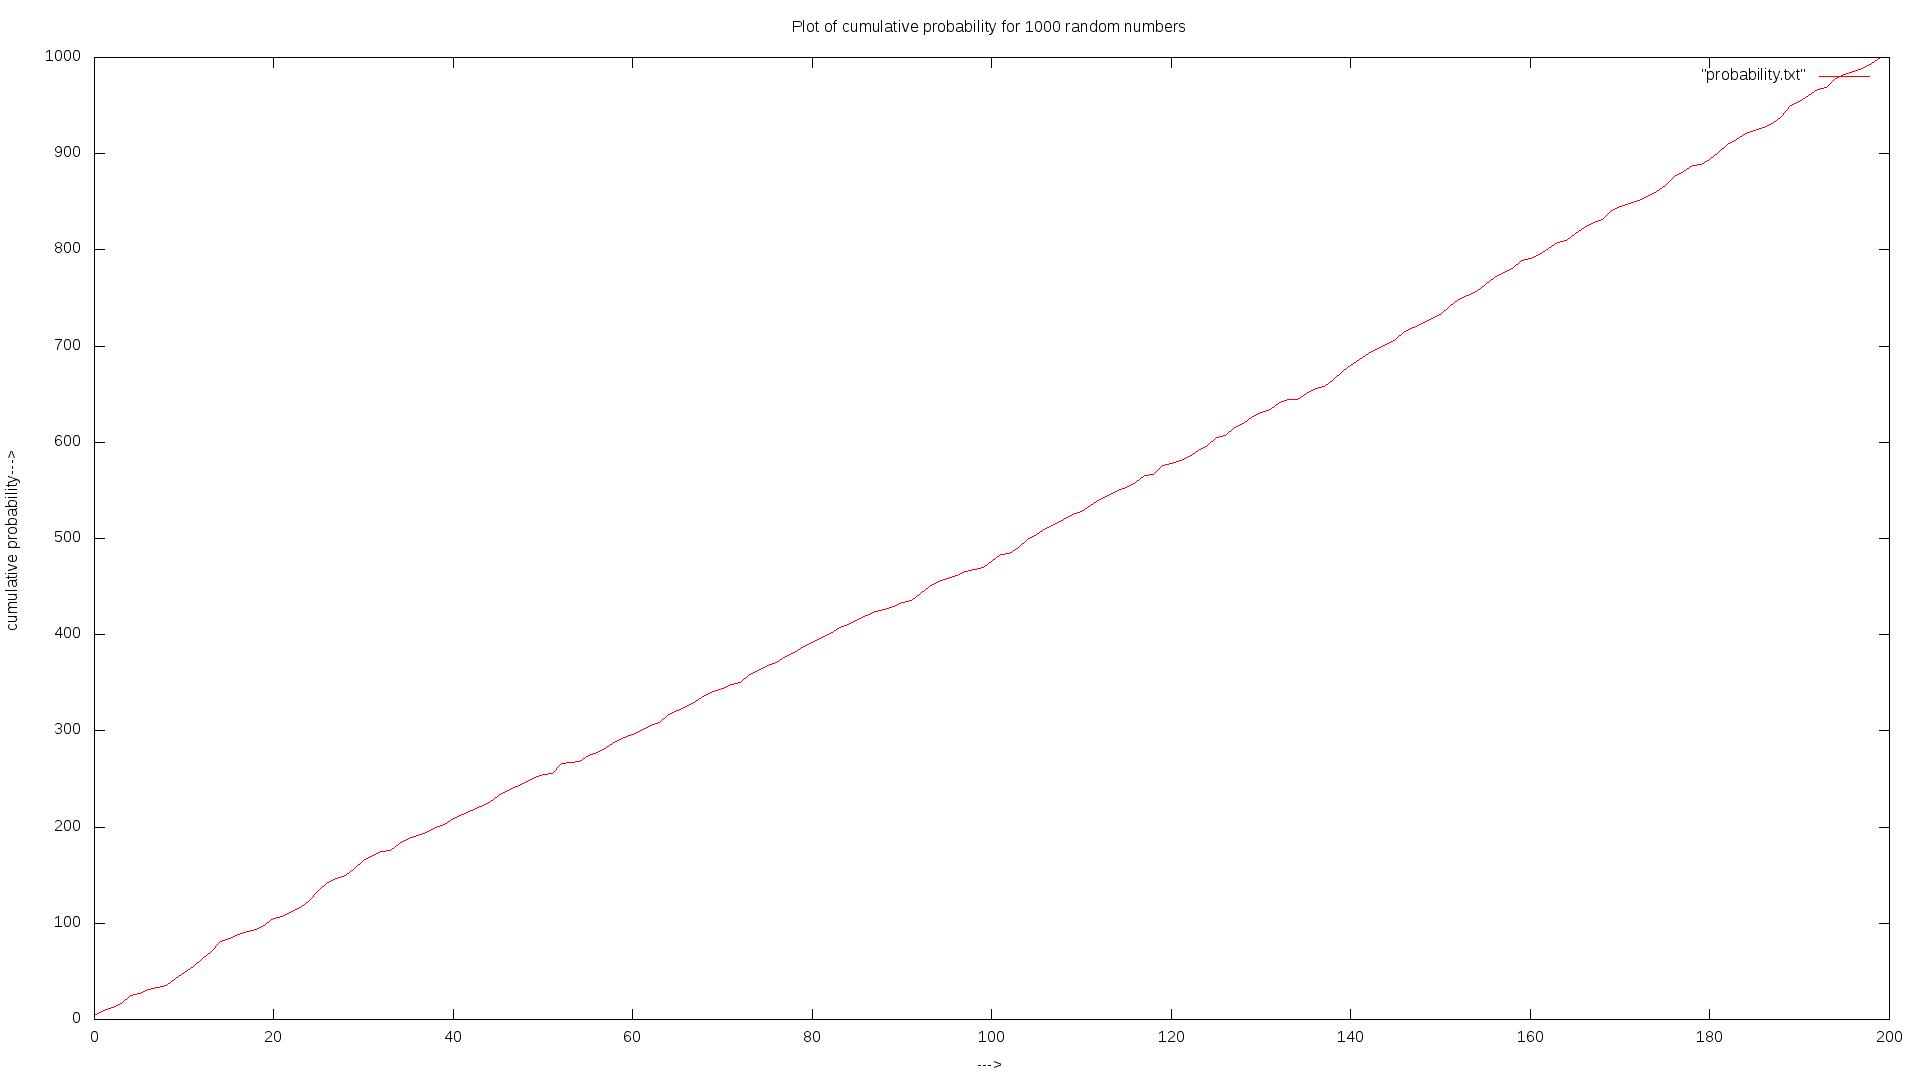
\includegraphics[width=1.0\textwidth]{q2_probability.png}}
	\caption{Plot of cumulative probability distribution for 1000 random numbers}
\end{figure}
\newpage
{\underline{Observations:}\\
\begin{itemize}
\item The sample means and variances seem to converge to a value as observed from the graphs and the output values.
\item The means converge to a value of 1072770038, and the variances converge to a value of 383718748000926080
\item The probability mass function (cumulative frequencies in specific intervals) of the random numbers is observed to be approximately a straight line, parallel to the line with slope 1.
\item This shows that the cummulative probability increases uniformly, resembling the probability mass function of the random variable unif(0,1).
\end{itemize}
\end{document}